\documentclass{article}
\usepackage{amsmath,amssymb,amsthm}
\usepackage{geometry}
\usepackage{siunitx}
\usepackage{mathtools}
\usepackage{hyperref} % Added for clickable citations and URL
\usepackage{graphicx} % For benchmark figures
\geometry{margin=1in}
% \linespread{1.4} % temp toggle for drafts
% === Theorem-like environments ===
\newtheorem{definition}{Definition}
\newtheorem{theorem}{Theorem}
\newtheorem{proposition}{Proposition}
\newtheorem{remark}{Remark}

\begin{document}

\begin{center}
 {\fontsize{18}{20}\selectfont\bfseries Radial Dual Lattice Graphs via Admissible Inversion: Exact Folding Operators for Eisenstein, Hurwitz, and $E_8$ Lattices}\\[1.2em]
Nathan O. Schmidt$^{1}$, Klee Irwin$^{2}$, and Natasha Urakhchina$^{2}$ \\[0.6em]
\textit{$^{1}$Cold Hammer Research \& Development LLC, Eagle, Idaho, USA} \\[0.1em]
\texttt{nate.o.schmidt@coldhammer.net}$^{1}$ \\[0.4em]
\textit{$^{2}$Quantum Gravity Research, Topanga, California, USA} \\[0.1em]
\texttt{klee@quantumgravityresearch.org}$^{2}$, \texttt{natasha@quantumgravityresearch.org}$^{2}$ \\[0.6em]
March 7, 2026
\end{center}

\begin{abstract}
On nearest-neighbor graphs of exceptional lattices that encode normed division algebras, we propose a framework that leverages admissible hyperspherical inversion to construct \emph{radial dual lattice graphs}. Beginning with the Eisenstein integers in 2D---as established by the Tri-Quarter Framework (TQF) \cite{Schmidt2025}---we extend the construction to the Hurwitz quaternion lattice in 4D and the $E_8$ lattice in 8D via recursive bootstrapping. At each dimensional level, the inversion induces graph isomorphisms between the outer zone and inner zone subgraphs that preserve adjacency, norms, radial directions, and symmetry groups to achieve discrete and reversible combinatorial self-dualities between the outer and inner zones. In 8D, this approach aims to equip Cycle Clock Theory (CCT) with an exact radial folding operator that maps arbitrarily large-norm cycle clocks on the $E_8$ lattice to compact inner zone equivalents in the rational extension. If successfully integrated into CCT workflows, such an operator may significantly reduce computational complexity for the simulation and enumeration of quasicrystalline dynamics while preserving all combinatorial invariants. Benchmarking demonstrates that the modular reduction induced by the radial dual delivers divisor-sum formulas for $E_8$ shell multiplicities with approximately $83\,000$\,--$260\,000\times$ speedups compared to traditional theta function polynomial expansions at moderate shell indices, where the advantage grows rapidly for larger increasing norms. Radial dual admissible hyperspherical inversion is composed with the Moxness $E_8$-to-$H_4$ matrix $H_{4\mathrm{fold}}$ to define the golden linear-radial dual compressor $\Upsilon_r$, which maps the 8D radial dual directly onto the 600-cell geometry and its golden-ratio scaled copy $H_4\Phi$ to achieve a precise dimensional reduction from 8D to 4D while maintaining all algebraic invariants. Realized via the Cayley integers in 8D, this framework aligns conceptually with octonion-based models in quasicrystalline quantum gravity. The construction remains strictly algebraic and geometric, operating on rational extensions without approximations, floating-point drift, continuous relaxations, or information loss. Moreover, it offers an exact algebraic tool that supports shelling and scaling analyses in CCT by enabling compact inner zone computations of shell multiplicities, orientation statistics, and number-theoretic decompositions. While the radial dual construction, induced lower-dimensional graph isomorphisms, coordinate compression, explicit cycle clock folding examples, and divisor-sum acceleration of shell multiplicities are rigorously established and numerically verified in this work, the full extension to 8D graph isomorphisms, comprehensive integration into CCT simulation pipelines, and large-norm cycle clock enumeration remain subjects for further investigation and validation.
\end{abstract}

\section{Introduction}
\label{sec:introduction}

The exceptional lattices associated with the normed division algebras stand in a unique and structurally inevitable position in mathematics, computer science, and theoretical physics. These structures emerge directly from the geometry of maximally dense sphere packings \cite{Viazovska2017,Cohn2021} in 1D, 2D, 4D, and 8D---the only dimensions that admit such algebras---which render the construction rigid and canonical instead of arbitrary.

This finite exceptional set of specific dimensional levels---which fundamentally terminates at 8D by the Hopf invariant one theorem of Adams \cite{Adams1960}---is precisely what facilitates the admissibility condition for inversion radii with its profound mathematical significance, while ensuring that the discrete symmetry-invariant shells enable exact bijective radial dualities throughout the recursive bootstrapping process.

This first principles work generalizes the Eisenstein integer based Tri-Quarter Framework (TQF) \cite{Schmidt2025} from 2D to 4D and 8D without sacrificing the exact discrete, rational, and efficient character of the original. We design and deploy \emph{radial dual lattice graphs} by driving admissible hyperspherical inversion straight through the nearest-neighbor graph of each exceptional lattice.

Hyperspherical inversion denotes the classical geometric transformation that inverts points with respect to a hypersphere of radius $r$ centered at the origin in $\mathbb{R}^n$. It is the direct higher-dimensional generalization of circular inversion in the plane and spherical inversion in 3D. Although these inversions have a long history in geometry---tracing to foundational contributions by Jakob Steiner in 1824 and systematically developed in the theory of inversive geometry \cite{MorleyMorley1933,Coxeter1969}---their specific application here to admissible radii determined by the norm form of exceptional lattices is novel. This application, which induces exact graph isomorphisms between the outer zone and inner zone subgraphs, begins from the original 2D radial dual graph construction \cite{Schmidt2025}.

The present framework is distinguished by its purely algebraic and geometric nature, while operating exclusively on rational extensions of the underlying exceptional lattices---with no approximations, floating-point drift, continuous relaxations, or information loss. The construction remains entirely within rational extensions of the lattices---this uncompromising exactness is its core advantage.

At each dimensional level of exception, the inversion map induces a graph isomorphism that preserves adjacency, norms, radial directions, and symmetry groups. For instance, as we demonstrate in this paper, the 8D radial dual equips Cycle Clock Theory (CCT) with an exact radial-folding operator that maps arbitrarily large-norm cycle clocks on the $E_8$ lattice to compact inner zone equivalents in the rational extension. This reduces computational complexity in the simulation and enumeration of quasicrystalline dynamics while preserving all combinatorial invariants. In this context, the present construction constitutes a direct algebraic assault on what is a great challenge of $E_8$-based modeling: the explosive growth in combinatorial scale and computational intractability encountered when simulating or enumerating quasicrystalline dynamics and cycle clocks at large radial norms on the $E_8$ lattice. The radial dual framework directly addresses this challenge by providing an exact reversible coordinate-compression and folding mechanism. In particular, computational verification shows that the associated modular substitution reduces $E_8$ shell-multiplicity computations from theta function polynomial expansions to simple divisor sums to achieve speedups of more than $80\,000\times$ at shell index $n=1\,000$ and over $260\,000\times$ at $n=2\,000$, where the advantage continues to scale favorably for increasingly large norms. The golden linear-radial dual compressor \(\Upsilon_r\), constructed by composing the Moxness $E_8$-to-$H_4$ matrix \(H_{4\mathrm{fold}}\) \cite{Moxness2014} with radial dual admissible hyperspherical inversion, maps the 8D radial dual directly onto the 600-cell geometry and its golden-ratio scaled copy \(H_4\Phi\) to achieve dimensional reduction while preserving all algebraic invariants and further enhancing computational efficiency in CCT applications. The framework aligns directly with octonion-based models through a realization via the Cayley integers (integral octonions) in 8D.

While the radial dual construction, induced graph isomorphisms, coordinate compression, explicit cycle clock folding, and divisor-sum acceleration of shell multiplicities are rigorously established in this work, their comprehensive application to full CCT simulations—including large-norm cycle clock enumeration, phason/gauge dynamics, and end-to-end projection pipelines—remains a goal for future investigation.

The paper is organized as follows:

\begin{itemize}
\item Section~\ref{sec:notation} establishes the general notation, standing assumptions, and definitions (including admissible radii and the hyperspherical inversion map) used throughout the work;
 \item Section~\ref{sec:2d-eisenstein} recaps the original 2D Eisenstein integer based radial dual lattice graph of the TQF \cite{Schmidt2025};
 \item Sections~\ref{sec:4d-bootstrapping} and~\ref{sec:bootstrapping-8d} bootstrap the construction recursively to the 4D Hurwitz quaternion lattice and the 8D $E_8$ lattice to prove the corresponding graph isomorphisms;
 \item Section~\ref{sec:h4-folding} introduces the complementary linear $H_4$ folding operator and its composition with radial inversion;
 \item Section~\ref{sec:cct-application} details the applications to CCT, which includes explicit cycle clock examples and connections to shelling and scaling analyses;
 \item Section~\ref{sec:computational-verification} reports comprehensive computational verification using exact arithmetic; and
 \item Section~\ref{sec:conclusion} concludes with implications and future directions.
\end{itemize}

With our intent and direction solidified, we proceed to drive the radial dual lattice graph construction, starting from the Eisenstein integers. But first, we introduce some generalized notation.

\section{Notation and Standing Assumptions}
\label{sec:notation}

Throughout this work we operate in Euclidean space $\mathbb{R}^d$ with squared norm $N(\cdot)$ for $d \in \{2,4,8\}$. Let $L^d$ denote the corresponding exceptional lattice (Eisenstein integers for $d=2$, Hurwitz quaternions for $d=4$, Cayley integers / $E_8$ root lattice for $d=8$). The punctured nearest-neighbor graph on $L^d \setminus \{0\}$ is denoted $\Lambda^d$.

Throughout this work, each element $\mathbf{v} \in L^d$ ($d=2,4,8$) is understood simultaneously as
\begin{itemize}
  \item a \emph{lattice point} in the exceptional lattice $L^d \subset \mathbb{R}^d$,
  \item a \emph{vertex} of the punctured nearest-neighbor graph $\Lambda^d$,
  \item and a \emph{vector} in Euclidean space $\mathbb{R}^d$.
\end{itemize}
We adopt the convention that the generic symbols $\mathbf{v}$ and $\mathbf{u}$ (together with their primed or indexed variants $\mathbf{v}'$, $\mathbf{u_i}$, etc.) refer interchangeably to these three equivalent objects when the element lies in $L^d$. For points in the rational extension $\mathbb{Q} \otimes L^d$ (in particular the inner zone $\Lambda_{-,r}^d$), we retain the same symbols $\mathbf{v}$ and $\mathbf{u}$ but understand them primarily as \emph{vertices} of the radial dual graph and as \emph{vectors} in $\mathbb{R}^d$, while no longer referring to them as lattice points of $L^d$. This convention is consistent with the notational practice established in the TQF \cite{Schmidt2025}.

\begin{definition}[Admissible inversion radius]
\label{def:admissible-inversion-radius}
Let $L^d \subset \mathbb{R}^d$ ($d=2,4,8$) be one of the exceptional lattices equipped with the squared Euclidean norm $N(\cdot)$. A radius $r > 0$ is said to be \emph{admissible} (with respect to $L^d$) if there exists a nonzero vector $\mathbf{v} \in L^d$ such that
\[
r^2 = N(\mathbf{v}).
\]
\end{definition}

For any admissible radius $r > 0$ (i.e., $r^2$ equals the squared norm of some nonzero lattice vector), let $S_r^{d-1}$ denote the hypersphere of radius $r$ centered at the (punctured) origin in $\mathbb{R}^d$. The vertex set of $\Lambda^d$ is partitioned into three disjoint zones:
\begin{itemize}
  \item \textbf{Outer zone}: $\Lambda_{+,r}^d = \{\mathbf{v} \in L^d \mid N(\mathbf{v}) > r^2\}$,
  \item \textbf{Boundary zone (threshold shell)}: $\Lambda_{T,r}^d = \{\mathbf{v} \in L^d \mid N(\mathbf{v}) = r^2\} = L^d \cap S_r^{d-1}$,
  \item \textbf{Inner zone}: $\Lambda_{-,r}^d = \iota_r(\Lambda_{+,r}^d) \subset \mathbb{Q} \otimes L^d$.
\end{itemize}

The inversion map is defined on nonzero vertices by
\[
\iota_r(\mathbf{v}) = \frac{r^2 \, \mathbf{v}}{N(\mathbf{v})}, \qquad \mathbf{v} \in \mathbb{R}^d \setminus \{0\}.
\]
This is the direct higher-dimensional generalization of circular inversion. In all dimensions it satisfies the following algebraic properties (verified by direct substitution into the definition):
\begin{enumerate}
  \item \textbf{Involution}: $\iota_r(\iota_r(\mathbf{v})) = \mathbf{v}$.
  \item \textbf{Boundary fixed set}: If $N(\mathbf{v}) = r^2$ then $\iota_r(\mathbf{v}) = \mathbf{v}$.
  \item \textbf{Zone swap}: $\iota_r(\Lambda_{+,r}^d) = \Lambda_{-,r}^d$ and vice versa.
  \item \textbf{Angular preservation}: $\arg(\iota_r(\mathbf{v})) = \arg(\mathbf{v})$; each vertex and its image live on the same radial ray from the origin.
  \item \textbf{Norm relation}: $N(\iota_r(\mathbf{v})) = r^4 / N(\mathbf{v})$.
\end{enumerate}

\begin{remark}[Adjacency norm identity (general)]
\label{rem:general-adjacency-identity}
Let \(\mathbf{u},\mathbf{v}\in\Lambda_{+,r}^d\) be adjacent, i.e., \(N(\mathbf{u}-\mathbf{v})=\delta\) where \(\delta\) is the squared length of the minimal vectors of the lattice (\(\delta=1\) for \(d=2,4\); \(\delta=2\) for \(d=8\)). Then
\[
N\bigl(\iota_r(\mathbf{u})-\iota_r(\mathbf{v})\bigr)=\frac{r^4\,\delta}{N(\mathbf{u})\,N(\mathbf{v})}.
\]
This follows by direct expansion:
\begin{align*}
\iota_r(\mathbf{u})-\iota_r(\mathbf{v})
&= r^2\left(\frac{\mathbf{u}}{N(\mathbf{u})} - \frac{\mathbf{v}}{N(\mathbf{v})}\right), \\
N(\iota_r(\mathbf{u})-\iota_r(\mathbf{v}))
&= r^4 \cdot \frac{N(\mathbf{u}-\mathbf{v})}{N(\mathbf{u})\,N(\mathbf{v})} = \frac{r^4\,\delta}{N(\mathbf{u})\,N(\mathbf{v})}.
\end{align*}
The identity quantifies how nearest-neighbor distances are transformed in the inner zone and is used in the computational verification of adjacency preservation.
\end{remark}

The adjacency norm identity is important to this framework because it demonstrates that admissible circular/spherical/hyperspherical inversion transforms nearest-neighbor edges from the outer zone to the inner zone in a precisely controlled algebraic manner: an outer zone edge of squared length \(\delta\) is mapped to an inner zone edge of squared length \(\frac{r^4 \delta}{N(\mathbf{u})N(\mathbf{v})}\). Since the scaling factor is always positive and only depends on the norms of the endpoints, the inversion map \(\iota_r\) preserves the combinatorial adjacency relation exactly, even as Euclidean distances are radially rescaled. This algebraic fact is foundational because it guarantees that \(\iota_r\) induces graph isomorphisms between the outer and inner zone subgraphs in all dimensions (Theorems~\ref{thm:2d-duality}, \ref{thm:4d-duality}, \ref{thm:8d-duality}), underpins the exact computational verification of the radial dual, and enables folding of arbitrarily large-norm cycle clocks into compact rational representations without information loss.

\begin{remark}
\label{rem:escher-visualization}
The geometric essence of the admissible hyperspherical inversion $\iota_r$ receives a striking artistic visualization in M.~C.~Escher's 1935 lithograph \emph{Hand with Reflecting Sphere} \cite{Escher1935}. In this self-portrait, a spherical mirror maps the surrounding room such that distant exterior points appear compressed near the center of the reflection (inner zone), while points near the mirror surface map outward, all along preserved radial rays and with local angle preservation. This intuitive depiction precisely captures the zone-swapping property, radial preservation, and conformal character of the transformation formalized above.
\end{remark}

The full radial dual lattice graph is $\Lambda_r^d$ with vertex set $\Lambda_{-,r}^d \cup \Lambda_{T,r}^d \cup \Lambda_{+,r}^d$ and edge set constructed exactly as in the 2D TQF (outer edges, inverted inner edges, and boundary-crossing edges).

Standing assumptions (used throughout this paper):
\begin{enumerate}
  \item The origin is excluded from all graphs and zone partitions, as hyperspherical inversion is undefined at the origin. (See Remark~\ref{rem:2d-graph-properties-2} below.)
  \item All constructions remain strictly inside the rational extension $\mathbb{Q} \otimes L^d$, with no approximations, floating-point drift, continuous relaxations, or information loss.
  \item Unless otherwise stated, the canonical admissible radius corresponding to the minimal positive norm shell is understood ($r=1$ for $d=2,4$; $r=\sqrt{2}$ for $d=8$).
\end{enumerate}

\begin{remark}
\label{rem:2d-graph-properties-2}
The exclusion of the origin is not merely a technical necessity that arises from the singularity of spherical inversion at zero. Rather, it constitutes a structurally enabling feature: puncturing the origin removes the unique fixed point under all radial scalings and inversions, which allows the inversion map $\iota_r$ to act as a free involution (with no fixed points outside the boundary shell) on the punctured lattice. This freedom unleashes a profound cascade of discrete symmetries and combinatorial dualities---most notably the exact bijective graph isomorphism between outer and inner zones---that would be obstructed if the origin were retained as a distinguished vertex. In this context, the punctured structure is foundational to the recursive bootstrapping of radial dual lattice graphs across exceptional dimensions and to the preservation of strict combinatorial self-duality under admissible inversion.
\end{remark}

\section{Tri-Quarter Framework in 2D: Eisenstein Radial Dual Lattice Graphs}
\label{sec:2d-eisenstein}

The original radial dual lattice graph construction is based on the Eisenstein integers in 2D via the TQF \cite{Schmidt2025}. It achieves an exact bijective duality---between $\Lambda_{+,r}^2$ and $\Lambda_{-,r}^2$---that is preserved under the graph structure and serves as the inductive base for the recursive bootstrapping to higher dimensions developed in this paper.

\subsection{Eisenstein Lattice Graph}
\label{subsec:2d-eisenstein-lattice}
Let $\omega = e^{2\pi i / 3} = -\frac{1}{2} + i \frac{\sqrt{3}}{2}$ be a primitive cube root of unity. The Eisenstein integers form the ring
\[
\mathbb{Z}[\omega] = \{ m + n\omega \mid m,n \in \mathbb{Z} \}.
\]
The associated lattice $L^2 \subset \mathbb{C} \cong \mathbb{R}^2$ is given by the explicit embedding
\[
\mathbf{v} = m + n\omega = \Bigl(m - \frac{n}{2}\Bigr) + i \frac{n\sqrt{3}}{2},
\]
with squared Euclidean norm
\[
N(\mathbf{v}) = m^2 - mn + n^2 \in \mathbb{N}_0.
\]
This quadratic form is positive definite and integer-valued on the lattice, and generates exact regular hexagonal shells of radius $\sqrt{k}$ for admissible integers $k$.

\begin{definition}
\label{def:2d-lattice-graph}
The \emph{underlying lattice graph} $\Lambda^2$ is the countably infinite undirected graph with
\begin{itemize}
  \item vertices: $L^2$,
  \item edges: pairs $\{\mathbf{v}, \mathbf{u}\}$ such that $N(\mathbf{v} - \mathbf{u}) = 1$ (nearest-neighbor minimal vectors).
\end{itemize}
\end{definition}

\begin{remark}
\label{rem:punctured-plane}
The TQF and the radial dual construction operate on the origin-punctured complex plane $\mathbb{C} \setminus \{0\} \cong \mathbb{R}^2 \setminus \{0\}$. Circular inversion is undefined only at the origin, and the origin vertex is therefore excluded from the zone partitioning and from the domain of the inversion map $\iota_r$ in order to preserve bijectivity and the discrete combinatorial structure of the radial dual lattice graph.
\end{remark}

\begin{remark}
\label{rem:2d-graph-properties}
The graph $\Lambda^2$ is the countably infinite triangular (hexagonal) grid graph on the punctured plane $\mathbb{R}^2 \setminus \{0\}$. Every vertex has degree 6, which corresponds to the six nearest neighbors separated by $60^\circ$ angular intervals. The full isometry group of the underlying lattice is the dihedral group $D_6$ of order 12, generated by $60^\circ$ rotations and reflections, which acts transitively on the nonzero lattice points and preserves the graph structure.
\end{remark}

\subsection{Admissible Inversion Radius in 2D}
\label{subsec:2d-admissible-inversion-radius}

Fix an admissible radius $r > 0$ as per Definition~\ref{def:admissible-inversion-radius}. The canonical choice is $r = 1$ (corresponding to $N = 1$), which produces the boundary zone $\Lambda_{T,r}^2 = L^2 \cap S_r^1$ containing exactly six vertices that form a regular hexagon centered at the origin.

The admissibility condition of Definition \ref{def:admissible-inversion-radius} guarantees that the boundary zone $\Lambda_{T,r}^d = L^d \cap S_r^{d-1}$ is a discrete, finite, and symmetry-invariant subset of $L^d$. This property ensures that the subsequent inversion map sends all vertices to well-defined vertices in the rational extension while preserving the discrete combinatorial structure required for the radial dual graph construction.

\subsection{Zone Partitioning and Circular Inversion in 2D}
\label{subsec:2d-zone-partitioning}
Fix an admissible radius $r > 0$. The inner zone will consist of the images of the outer zone vertices under the circular inversion map $\iota_r : \mathbb{C} \setminus \{0\} \to \mathbb{C} \setminus \{0\}$ that we define explicitly in the next subsection. Then we partition the vertex set of $\Lambda^2 \setminus \{0\}$ into three disjoint subsets:
\begin{itemize}
  \item \textbf{Outer zone}: $\Lambda_{+,r}^2 = \{ \mathbf{v} \in L^2 \mid N(\mathbf{v}) > r^2 \}$,
  \item \textbf{Boundary zone}: $\Lambda_{T,r}^2 = \{ \mathbf{v} \in L^2 \mid N(\mathbf{v}) = r^2 \} = L^2 \cap S_r^1$,
  \item \textbf{Inner zone}: $\Lambda_{-,r}^2 = \iota_r(\Lambda_{+,r}^2)$, the set of all vertices in $\mathbb{Q}(\omega)$ obtained by inversion (generally with rational coefficients in the Eisenstein basis).
\end{itemize}
The full radial dual lattice graph $\Lambda_r^2$ is the undirected graph with
\begin{itemize}
  \item vertex set is the disjoint union $V(\Lambda_r^2) = \Lambda_{-,r}^2 \cup \Lambda_{T,r}^2 \cup \Lambda_{+,r}^2$,
  \item edge set consists of (i) the outer zone nearest-neighbor edges of $\Lambda^2$, (ii) their images under $\iota_r$ in the inner zone, and (iii) crossing edges connecting boundary vertices to inverted outer vertices (defined precisely in the next subsection).
\end{itemize}
The vertices of $\Lambda_{-,r}^2$ reside in $\mathbb{Q}(\omega)$, and therefore generally carry rational (rather than integer) coefficients in the Eisenstein basis.

This partitioning creates a tripartite (or ``Tri-Quarter'') division of the punctured plane $\mathbb{C} \setminus \{0\}$: the outer zone $\Lambda_{+,r}^2$ consists of all lattice vertices with $N(\mathbf{v}) > r^2$ (beyond the boundary shell), the boundary zone $\Lambda_{T,r}^2 = L^2 \cap S_r^1$ comprises the fixed admissible shell $N(\mathbf{v}) = r^2$, and the inner zone $\Lambda_{-,r}^2$ is the exact algebraic image of $\Lambda_{+,r}^2$ under inversion of $\iota_r$ through the circle $S_r^1$ of radius $r$.

The inversion map $\iota_r$ is given in Section~\ref{sec:notation} and satisfies the five algebraic properties listed there. In the context of the Eisenstein lattice $L^2$ and the TQF \cite{Schmidt2025,SchmidtTriQuarterGeneral}, the map is conformal and angle-preserving, thereby respecting the $60^\circ$ angular structure inherent to the triangular lattice $L^2$.

Geometrically, $\iota_r$ radially rescales every vertex $\mathbf{v} \in \Lambda_{r}^2$ through the circle $S_r^1$ of radius $r$: any vertex $\mathbf{v} \in \Lambda_{+,r}^2$ that exists far outside the boundary $\Lambda_{T,r}^2$ is mapped to $\mathbf{v}' = \iota_r(\mathbf{v}) \in \Lambda_{-,r}^2$, which is close to the origin along the same radial ray, and vice versa. Because the map acts as a positive scalar multiple of the identity on each ray, it preserves radial directions and the discrete structure required for the radial dual lattice graph construction \cite{Schmidt2025}.

\subsection{Construction and Duality in 2D}
\label{subsec:2d-graph-construction-duality}
The edge set $E(\Lambda_r^2)$ of the radial dual lattice graph is defined in three parts:
\begin{itemize}
  \item \textbf{Outer zone edges}: all nearest-neighbor edges of $\Lambda^2$ with both endpoints in $\Lambda_{+,r}^2$,
  \item \textbf{Inner zone edges}: the images $\{\iota_r(\mathbf{v}), \iota_r(\mathbf{u})\}$ of every outer zone edge $\{\mathbf{v}, \mathbf{u}\}$,
  \item \textbf{Boundary crossing edges}: for each pair consisting of a boundary vertex $\mathbf{v} \in \Lambda_{T,r}^2$ and an outer vertex $\mathbf{u} \in \Lambda_{+,r}^2$ that are adjacent in $\Lambda^2$, add the edge $\{\mathbf{v}, \iota_r(\mathbf{u})\}$.
\end{itemize}

\begin{theorem}[2D Bijective Radial Graph Duality \cite{Schmidt2025}]
\label{thm:2d-duality}
For any admissible $r$, the restriction of $\iota_r$ induces a graph isomorphism
\[
\iota_r \colon (\Lambda_{+,r}^2, E(\Lambda_r^2)|_{\Lambda_{+,r}^2}) \;\to\; (\Lambda_{-,r}^2, E(\Lambda_r^2)|_{\Lambda_{-,r}^2}).
\]
\end{theorem}

\begin{proof}
The map $\iota_r$ is an algebraic involution that swaps $\Lambda_{+,r}^2$ and $\Lambda_{-,r}^2$ bijectively. By construction of the edge set, every outer zone nearest-neighbor edge maps directly to an inner zone edge. Boundary-crossing edges are mirrored symmetrically via the involution property and fixed boundary.

The dihedral symmetry group $D_6$ commutes with $\iota_r$ because circular inversion through an origin-centered admissible shell is conformal and angle-preserving, and the lattice is $D_6$-invariant. Therefore $\iota_r$ is a graph isomorphism between the induced subgraphs (see also Remark \ref{rem:2d-graph-properties}).
\end{proof}

\begin{figure}[htbp]
\centering
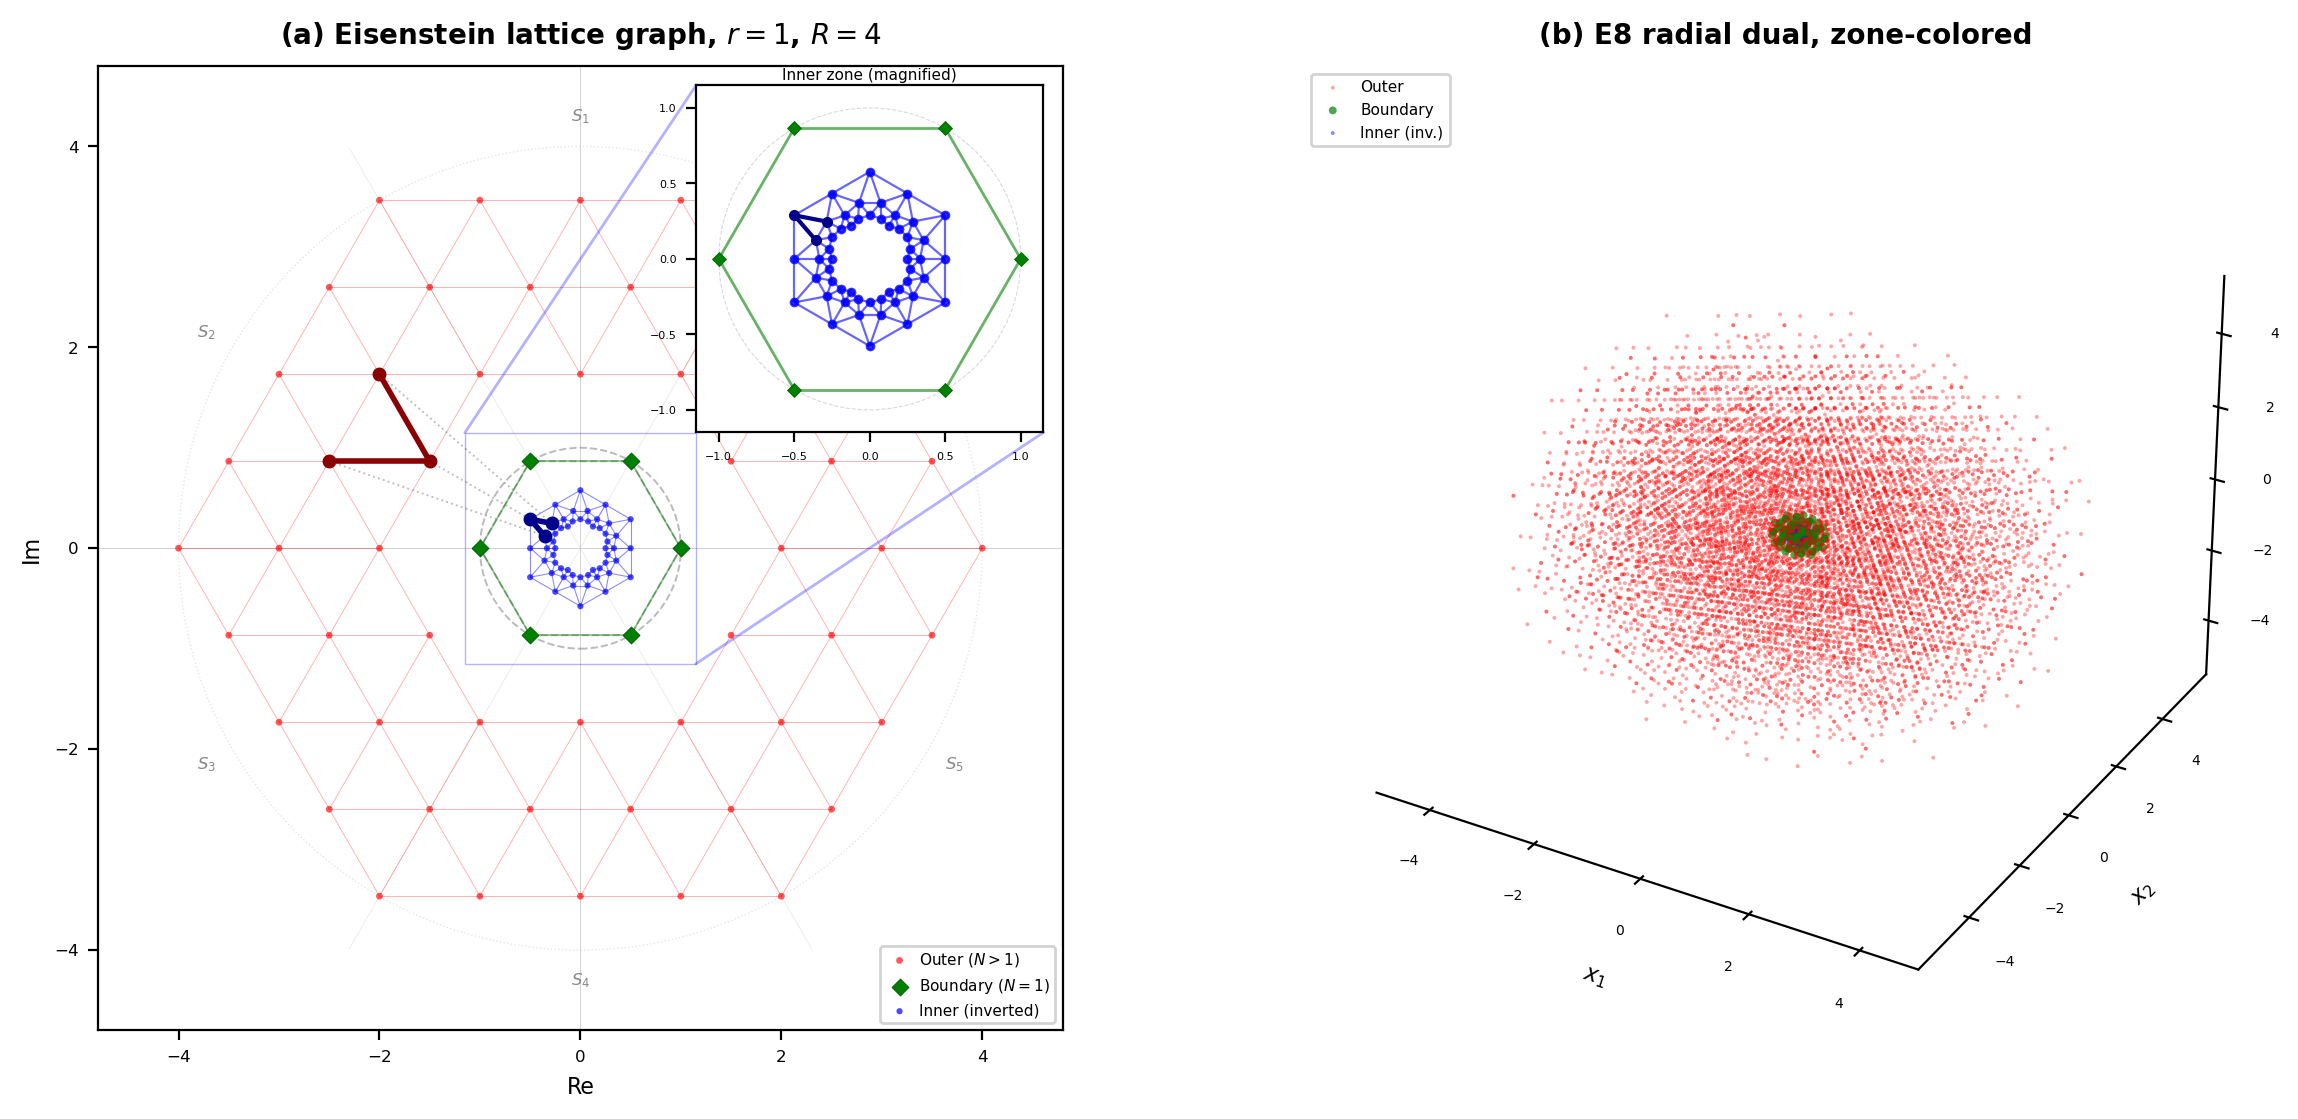
\includegraphics[width=\textwidth]{radial_dual_lattice_graphs.png}
\caption{Radial dual lattice graphs with zone-colored edges. \textbf{(a)} Eisenstein lattice graph with $r=1$, $R=4$. Red/blue edges show the graph isomorphism between $\Lambda_{+,r}^2$ and $\Lambda_{-,r}^2$ (boundary shell $\Lambda_{T,r}^2 = L^2 \cap S_r^1$). Inset: magnified $\Lambda_{-,r}^2$. \textbf{(b)} $E_8$ radial dual projected to 3D via $H_{4\mathrm{fold}}$, inversion, and FIG slice, zone-colored to match.}
\label{fig:radial-dual-lattice-graph}
\end{figure}
Having established the foundational 2D case via the TQF and verified its exact bijective radial duality in Theorem \ref{thm:2d-duality}, we now extend the construction recursively to the next exceptional dimension by bootstrapping from the Eisenstein integers to the Hurwitz quaternions.

\section{Bootstrapping to 4D: Radial Dual Hurwitz Quaternion Lattice Graphs}
\label{sec:4d-bootstrapping}
The construction and proof that were established for the Eisenstein integers in 2D extend verbatim to the Hurwitz quaternion lattice in 4D. The admissible hyperspherical inversion \(\iota_r\) induces an exact graph isomorphism between the outer zone and inner zone induced subgraphs while preserving adjacency, norms, radial directions, and the binary tetrahedral symmetry group \(2T\).

\subsection{Hurwitz Quaternion Lattice Graph}
\label{subsec:4d-hurwitz-lattice}
Quaternions extend the complex numbers from 2D to 4D and furnish a natural algebraic environment for rotations in 3D space. The Hurwitz integers form the densest lattice packing in 4D. They comprise all quaternions
\[
\mathbf{q} = a + bi + cj + dk, \quad a,b,c,d \in \tfrac{1}{2}\mathbb{Z},
\]
such that \(a+b+c+d \in \mathbb{Z}\). The associated lattice \(L^4 \subset \mathbb{R}^4\) carries the norm \(N(\mathbf{q}) = a^2 + b^2 + c^2 + d^2\).

\begin{definition}
\label{def:4d-lattice-graph}
The \emph{underlying lattice graph} \(\Lambda^4\) is the countably infinite undirected graph with
\begin{itemize}
  \item vertices: \(L^4\),
  \item edges: pairs \(\{\mathbf{q}, \mathbf{p}\}\) such that \(N(\mathbf{q} - \mathbf{p}) = 1\) (nearest-neighbor minimal vectors).
\end{itemize}
\end{definition}
Each vertex has degree 24 to match the 24 units of \(\mathbb{H}\).

\subsection{Admissible Inversion Radius in 4D}
\label{subsec:4d-admissible-inversion-radius}
Fix an admissible radius $r > 0$ as per Definition~\ref{def:admissible-inversion-radius}. The canonical choice $r = 1$ yields the boundary zone $\Lambda_{T,r}^4 = L^4 \cap S_r^3$ containing the 24 vertices of squared norm 1, which form the vertex set of the regular 24-cell.

Admissibility guarantees that the boundary zone $\Lambda_{T,r}^4 = L^4 \cap S_r^3$ is a discrete, finite, and symmetry-invariant subset of $L^4$.

\subsection{Zone Partitioning and Hyperspherical Inversion in 4D}
\label{subsec:4d-zone-partitioning}
The same tripartite division applied in 2D extends directly to 4D. Thus, we prepare for an inductive transfer of the bijective duality established in Theorem \ref{thm:2d-duality}.

Fix an admissible radius \(r > 0\). The inner zone will consist of the images of the outer zone vertices under the hyperspherical inversion map $\iota_r : \mathbb{H} \setminus \{0\} \to \mathbb{H} \setminus \{0\}$ that we define explicitly in the next subsection. Partition the vertex set of \(\Lambda^4 \setminus \{0\}\) into three disjoint subsets exactly as in the 2D case:
\begin{itemize}
  \item \textbf{Outer zone}: \(\Lambda_{+,r}^4 = \{ \mathbf{q} \in L^4 \mid N(\mathbf{q}) > r^2 \}\),
  \item \textbf{Boundary zone}: \(\Lambda_{T,r}^4 = \{ \mathbf{q} \in L^4 \mid N(\mathbf{q}) = r^2 \} = L^4 \cap S_r^3\),
  \item \textbf{Inner zone}: \(\Lambda_{-,r}^4 = \iota_r(\Lambda_{+,r}^4)\), the set of all vertices in the rational extension \(\mathbb{Q} \otimes_{\mathbb{Z}} \mathbb{H}\) obtained by inversion.
\end{itemize}
The full radial dual lattice graph $\Lambda_r^4$ is the undirected graph with
\begin{itemize}
  \item vertex set is the disjoint union $V(\Lambda_r^4) = \Lambda_{-,r}^4 \cup \Lambda_{T,r}^4 \cup \Lambda_{+,r}^4$,
  \item edge set consists of (i) the outer zone nearest-neighbor edges of $\Lambda^4$, (ii) their images under $\iota_r$ in the inner zone, and (iii) crossing edges connecting boundary vertices to inverted outer vertices (defined precisely in the next subsection).
\end{itemize}
The vertices of $\Lambda_{-,r}^4$ reside in the rational extension $\mathbb{Q} \otimes_{\mathbb{Z}} \mathbb{H}$, and therefore generally carry rational (rather than half-integer) coefficients in the Hurwitz basis.

The inversion map $\iota_r$ is given in Section~\ref{sec:notation} and satisfies the five algebraic properties listed there. This is the direct 4D analogue of the circular inversion in 2D: each vertex is reflected through $S_r^3$ with radius $r$ centered at the origin. Consequently, vertices that exist far outside the boundary shell are mapped close to the origin along the identical radial ray, and vice versa.

The map remains conformal and commutes with the natural action of $\mathrm{SU}(2) \times \mathrm{SU}(2)$ on $\mathbb{H}$, thereby preserving the angular and combinatorial structure required for the radial dual lattice graph construction.

\subsection{Construction and Duality in 4D}
\label{subsec:4d-graph-construction-duality}
The edge set \(E(\Lambda_r^4)\) of the radial dual lattice graph is defined exactly as in the 2D case:
\begin{itemize}
  \item \textbf{Outer zone edges}: all nearest-neighbor edges of \(\Lambda^4\) with both endpoints in \(\Lambda_{+,r}^4\),
  \item \textbf{Inner zone edges}: the images \(\{\iota_r(\mathbf{q}),\iota_r(\mathbf{p})\}\) of every outer zone edge \(\{\mathbf{q},\mathbf{p}\}\),
  \item \textbf{Boundary crossing edges}: for each pair consisting of a boundary vertex \(\mathbf{p} \in \Lambda_{T,r}^4\) and an outer vertex \(\mathbf{q}\in\Lambda_{+,r}^4\) that are adjacent in \(\Lambda^4\), add the edge \(\{\mathbf{p},\iota_r(\mathbf{q})\}\).
\end{itemize}

\begin{remark}[Adjacency norm identity in 4D]
\label{rem:adj-norm-identity-4d}
With canonical radius $r=1$ ($\Rightarrow r^4=1$) and minimal squared length $\delta=1$, Remark \ref{rem:general-adjacency-identity} specializes to
\[
N\bigl(\iota_r(\mathbf{q}) - \iota_r(\mathbf{p})\bigr) = \frac{1}{N(\mathbf{q})\,N(\mathbf{p})}
\]
for any adjacent vertices $\mathbf{p},\mathbf{q} \in \Lambda_{+,r}^4$.
\end{remark}

\begin{theorem}[4D Bijective Radial Graph Duality]
\label{thm:4d-duality}
For any admissible \(r\), the restriction of \(\iota_r\) induces a graph isomorphism
\[
\iota_r\colon(\Lambda_{+,r}^4,E(\Lambda_r^4)|_{\Lambda_{+,r}^4})\to(\Lambda_{-,r}^4,E(\Lambda_r^4)|_{\Lambda_{-,r}^4}).
\]
\end{theorem}
\begin{proof}
The map \(\iota_r\) is an algebraic involution that swaps \(\Lambda_{+,r}^4$ and \(\Lambda_{-,r}^4\) bijectively. By construction of the edge set, every outer zone nearest-neighbor edge maps directly to an inner zone edge. Boundary-crossing edges are mirrored symmetrically via the involution property and fixed boundary.

The order-24 binary tetrahedral group \(2\mathcal{T}\) commutes with \(\iota_r\) because hyperspherical inversion through an origin-centered admissible shell is equivariant under the natural action of \(\mathrm{SU}(2)\times\mathrm{SU}(2)\) on \(\mathbb{H}\). Therefore \(\iota_r\) is a graph isomorphism between the induced subgraphs.
\end{proof}

The natural symmetry group that acts on the Hurwitz quaternion lattice \(L^4\) (and therefore on the radial dual lattice graph \(\Lambda_r^4\)) is the order-24 binary tetrahedral group \(2\mathcal{T}\). This group commutes with \(\iota_r\) because the admissible inversion radius is origin-centered and the map \(\iota_r\) is equivariant under left--right unit multiplications on \(\mathbb{H}\).

\begin{remark}[Orthogonal splicing (2D to 4D)]
\label{rem:orthogonal-splicing-2d-4d}
An alternative view of the same duality may be obtained by orthogonally embedding each 2D dual pair $(\mathbf{v}_+, \iota_r(\mathbf{v}_+))$, where $\mathbf{v}_+ \in \Lambda_{+,r}^2$, as the quaternion
\[
\mathbf{q} = \mathbf{v}_+ + \iota_r(\mathbf{v}_+) j \in \mathbb{Q} \otimes_{\mathbb{Z}} \mathbb{H}.
\]
The resulting graph is isomorphic to a (non-canonical) subgraph of the full 4D radial dual $\Lambda_r^4$ and illustrates the recursive lifting of the 2D structure, but the canonical construction used throughout this paper operates directly on the Hurwitz lattice $L^4$.
\end{remark}

Now that we've verified that the radial dual lattice graph construction and the induced bijective graph isomorphism extend verbatim from the Eisenstein integers in 2D to the Hurwitz quaternions in 4D, we now proceed to the final exceptional dimension.

\section{Bootstrapping to 8D: Radial Dual $E_8$ Lattice Graphs}
\label{sec:bootstrapping-8d}
The construction and proof established for the Eisenstein integers in 2D and the Hurwitz quaternions in 4D extend verbatim to the $E_8$ root lattice in 8D. The admissible hyperspherical inversion \(\iota_r\) induces an exact graph isomorphism between the outer zone and inner zone induced subgraphs while preserving adjacency, norms, radial directions, and the full Weyl group symmetry $W(E_8)$.

\subsection{$E_8$ Lattice Graph}
\label{subsec:8d-e8-lattice}
The $E_8$ root lattice $L^8 \subset \mathbb{R}^8$ is the unique (up to isomorphism) even unimodular lattice in 8D. In the standard coordinate realization it consists of all vectors $\mathbf{x} = (\mathbf{x}_1,\dots,\mathbf{x}_8) \in \mathbb{Z}^8 \cup (\mathbb{Z}+\tfrac{1}{2})^8$ whose coordinate sum is even. Equivalently, it arises from pairs of Hurwitz quaternions $(\mathbf{p},\mathbf{q}) \in \mathbb{H}^2$ satisfying the gluing condition $\mathbf{p}+\mathbf{q} \in (1+i)\mathbb{H}$. The lattice is even (all squared norms are even integers) and self-dual ($L^8 = (L^8)^*$). It realizes the densest known sphere packing in $\mathbb{R}^8$.

Its $240$ vectors of squared Euclidean norm $2$---the roots---split into $112$ vectors of $\mathcal{D}_8$ ``checkerboard'' sub-lattice type ($\pm \mathbf{e}_i \pm \mathbf{e}_j$, $i<j$) and $128$ half-integer vectors ($\pm \tfrac{1}{2},\dots,\pm \tfrac{1}{2}$) with an even number of minus signs. These minimal vectors generate the $E_8$ root system and achieve the kissing number $240$.

\begin{definition}
\label{def:8d-lattice-graph}
The \emph{underlying lattice graph} $\Lambda^8$ is the countably infinite undirected graph with
\begin{itemize}
  \item vertices: $L^8$,
  \item edges: pairs $\{\mathbf{x}, \mathbf{y}\}$ such that $N(\mathbf{x} - \mathbf{y}) = 2$ (nearest-neighbor minimal vectors).
\end{itemize}
\end{definition}
Each vertex has degree $240$. The full isometry group of $L^8$ is the Weyl group $W(E_8)$ of order $696\,729\,600$, which acts transitively on the roots and preserves the graph structure.

\subsection{Octonionic Realization via Cayley Integers}
\label{subsec:8d-octonionic-realization}
The $E_8$ root lattice $L^8$ admits a canonical realization as the lattice of \emph{Cayley integers} (also known as integral octonions \cite{Baez2002} or the Dickson--Coxeter order) inside the real division algebra $\mathbb{O}$ of octonions. In the normalization used throughout this paper, where the minimal vectors satisfy $N(\mathbf{x}) = 2$, the lattice $L^8$ contains all Cayley integers with even norm, and the admissible boundary zone $\Lambda_{T,r}^8 = L^8 \cap S_r^7$ (with $r = \sqrt{2}$) consists precisely of the $240$ units with norm $2$.

Now the radial dual lattice graph construction never invokes octonion multiplication. Instead, it relies solely on the Euclidean quadratic form $N(\cdot)$ and ordinary radial scaling $\mathbf{x} \mapsto \lambda \mathbf{x}$ ($\lambda \in \mathbb{Q}_{>0}$), both of which remain well-defined and associative over \(\mathbb{R}\). Consequently, every operation stays inside the rational extension \(\mathbb{Q} \otimes_{\mathbb{Z}} L^8\) and admits exact finite-precision arithmetic. All algebraic properties established in lower dimensions (involution, zone swapping, norm relation, angular preservation, and symmetry commutation) hold verbatim on this structure. The vertices of \(\Lambda_{-,r}^8\) lie in the rational octonions \(\mathbb{Q} \otimes_{\mathbb{Z}} \mathbb{O}\), where they uphold discreteness, countability, and the bijective graph isomorphism of Theorem~\ref{thm:8d-duality}.

\begin{remark}[Octonionic coordinate embedding of $E_8$ with native CCT integration]
\label{rem:cayley-cct-alignment}
The standard construction of the $E_8$ root lattice as the set of Cayley integers (i.e., integral octonions) solidifies a natural conceptual link to the octonion-based models employed in CCT and related emergence programs \cite{Dixon1994,Furey2016}. This link is achieved while fully persisting the exact discrete, rational, and reversible character that constitutes the central strength of the present framework. In particular, the construction seamlessly integrates with CCT’s deliberate choice of the associative Clifford algebra $\mathrm{Cl}(8)$ as its primary operational algebra. Consequently, the Cayley integers serve as a distinct trustworthy coordinate vertex set that encodes both the exceptional geometry of the $E_8$ root lattice $L^8$ and its maximal symmetry group $W(E_8)$.
\end{remark}

\subsection{Admissible Inversion Radius in 8D}
\label{subsec:8d-admissible-inversion-radius}
Fix an admissible radius $r > 0$ as per Definition~\ref{def:admissible-inversion-radius}. The canonical and optimal choice is $r = \sqrt{2}$ (corresponding to $N = 2$, the root shell), which exactly coincides with the boundary zone $\Lambda_{T,r}^8 = L^8 \cap S_r^7$ containing the 240 roots.

The admissibility condition of Definition \ref{def:admissible-inversion-radius} guarantees that the boundary zone $\Lambda_{T,r}^8 = L^8 \cap S_r^7$ is a discrete, finite, and symmetry-invariant subset of $L^8$. This property ensures that the subsequent inversion map sends all vertices to well-defined vertices in the rational extension while maintaining the discrete combinatorial structure that is required to construct the radial dual graph.

This shell is invariant under the full Weyl group $W(E_8)$. Higher admissible shells (e.g., $N=4$) yield larger boundary sets but at the expense of symmetry reduction, and are therefore suboptimal for the radial dual construction because they would weaken the commutation of \(\iota_r\) with the full symmetry group used in Theorem \ref{thm:8d-duality}. In this first principles approach, we wish to maximize symmetry exploitation.

\subsection{Zone Partitioning and Hyperspherical Inversion in 8D}
\label{subsec:8d-zone-partitioning}
Fix an admissible radius $r > 0$. Just as in the 2D and 4D environments, the origin remains excluded (Remark \ref{rem:punctured-plane}). Hence, inversion map $\iota_r$ is rendered well-defined on all nonzero lattice points.

The inner zone consists of the images of the outer zone vertices under the hyperspherical inversion map $\iota_r : \mathbb{R}^8 \setminus \{0\} \to \mathbb{R}^8 \setminus \{0\}$. We partition the vertex set of \(\Lambda^8 \setminus \{0\}\) into three disjoint subsets:
\begin{itemize}
  \item \textbf{Outer zone}: $\Lambda_{+,r}^8 = \{\mathbf{x} \in L^8 \mid N(\mathbf{x}) > r^2 \}$,
  \item \textbf{Boundary zone}: $\Lambda_{T,r}^8 = \{\mathbf{x} \in L^8 \mid N(\mathbf{x}) = r^2 \} = L^8 \cap S_r^7$,
  \item \textbf{Inner zone}: $\Lambda_{-,r}^8 = \iota_r(\Lambda_{+,r}^8) \subset \mathbb{Q} \otimes L^8$,
\end{itemize}
where admissibility of $r$ ensures that every vertex in \(\Lambda_{+,r}^8\) is sent to a well-defined vertex in the rational extension \(\mathbb{Q} \otimes L^8\), and the image set remains discrete and countable.

The full radial dual lattice graph $\Lambda_r^8$ is the undirected graph with
\begin{itemize}
  \item vertex set is the disjoint union $V(\Lambda_r^8) = \Lambda_{-,r}^8 \cup \Lambda_{T,r}^8 \cup \Lambda_{+,r}^8$,
  \item edge set consists of (i) the outer zone nearest-neighbor edges of $\Lambda^8$, (ii) their images under $\iota_r$ in the inner zone, and (iii) crossing edges connecting boundary vertices to inverted outer vertices (defined precisely in the next subsection).
\end{itemize}
The vertices of $\Lambda_{-,r}^8$ reside in the rational extension $\mathbb{Q} \otimes L^8$, and therefore generally carry rational coefficients in the $E_8$ coordinate basis.

The inversion map \(\iota_r\) is given in Section~\ref{sec:notation} and satisfies the five algebraic properties listed there. This is the direct higher-dimensional analogue of circular inversion in 2D and hyperspherical inversion in 4D: each vertex is reflected through the origin-centered hypersphere \(S_r^7\) of radius \(r\), which sends distant vertices close to the origin (and vice versa) while preserving the ray from the origin on which the vertex lives.

No octonionic conjugation is involved because the transformation is simply a positive rational scaling of the vector \(\mathbf{x}\) itself. All operations therefore remain well-defined and associative over the reals, and the vertices of the inner zone \(\Lambda_{-,r}^8\) lie in the rational extension \(\mathbb{Q} \otimes L^8\) while preserving discreteness and countability.

These properties are directly exploited in the inductive proof of the 8D graph isomorphism (Theorem~\ref{thm:8d-duality}) and the adjacency norm identity (Remark~\ref{rem:adj-norm-identity-4d}).

\subsection{Construction and Duality in 8D}
\label{subsec:8d-graph-construction-duality}
The edge set \(E(\Lambda_r^8)\) of the radial dual lattice graph is defined exactly as in the 2D and 4D cases:
\begin{itemize}
  \item \textbf{Outer zone edges}: all nearest-neighbor edges of \(\Lambda^8\) with both endpoints in \(\Lambda_{+,r}^8\),
  \item \textbf{Inner zone edges}: the images \(\{\iota_r(\mathbf{x}),\iota_r(\mathbf{y})\}\) of every outer zone edge \(\{\mathbf{x},\mathbf{y}\}\),
  \item \textbf{Boundary crossing edges}: for each pair consisting of a boundary vertex \(\mathbf{y} \in \Lambda_{T,r}^8\) and an outer vertex \(\mathbf{x}\in\Lambda_{+,r}^8\) that are adjacent in \(\Lambda^8\), add the edge \(\{\mathbf{y},\iota_r(\mathbf{x})\}\).
\end{itemize}

\begin{theorem}[8D Bijective Radial Graph Duality]
\label{thm:8d-duality}
For any admissible \(r\), the restriction of \(\iota_r\) induces a graph isomorphism
\[
\iota_r\colon(\Lambda_{+,r}^8,E(\Lambda_r^8)|_{\Lambda_{+,r}^8})\to(\Lambda_{-,r}^8,E(\Lambda_r^8)|_{\Lambda_{-,r}^8}).
\]
\end{theorem}
\begin{proof}
The map \(\iota_r\) is an algebraic involution that swaps \(\Lambda_{+,r}^8\) and \(\Lambda_{-,r}^8\) bijectively. By construction of the edge set, every outer zone nearest-neighbor edge maps directly to an inner zone edge. Boundary-crossing edges are mirrored symmetrically via the involution property and fixed boundary.
The Weyl group \(W(E_8)\) commutes with \(\iota_r\) because (i) the admissible shell is origin-centered, (ii) \(L^8\) is self-dual, and (iii) central inversion \(\mathbf{x}\mapsto -\mathbf{x}\) (already in \(W(E_8)\)) is compatible with radial scaling along every ray. Consequently, the restriction of \(\iota_r\) is equivariant under \(W(E_8)\), ensuring that it induces a graph isomorphism preserving adjacency, radial directions, norms, and all combinatorial invariants of the lattice graph.
\end{proof}

The full isometry group of the $E_8$ root lattice \(L^8\) (and therefore of the radial dual lattice graph \(\Lambda_r^8\)) is the Weyl group \(W(E_8)\) of order $696\,729\,600$. This group commutes with \(\iota_r\) for the canonical admissible radius \(r=\sqrt{2}\) because the inversion is equivariant under all lattice isometries that fix the origin.

\begin{remark}[Orthogonal splicing (4D to 8D)]
\label{rem:orthogonal-splicing-4d-8d}
An alternative view of the same duality may be obtained by orthogonally embedding each 4D dual pair \((\mathbf{q}_+,\iota_r(\mathbf{q}_+))\), where \(\mathbf{q}_+ \in \Lambda_{+,r}^4\), as the Cayley integer
\[
\mathbf{x} = \mathbf{q}_+ + \iota_r(\mathbf{q}_+) \ell \in \mathbb{Q} \otimes_{\mathbb{Z}} \mathbb{O},
\]
where \(\ell\) is a suitable imaginary octonion unit orthogonal to the quaternion subalgebra. The resulting graph is isomorphic to a (non-canonical) subgraph of the full 8D radial dual \(\Lambda_r^8\) and illustrates the recursive lifting of the 4D structure, but the canonical construction used throughout this paper operates directly on the $E_8$ root lattice \(L^8\).
\end{remark}

\begin{remark}[Adjacency norm identity in 8D]
\label{rem:adj-norm-identity-8d}
With canonical radius $r=\sqrt{2}$ ($\Rightarrow r^4=4$) and minimal squared length $\delta=2$, Remark \ref{rem:general-adjacency-identity} specializes to
\[
N\bigl(\iota_r(\mathbf{x}) - \iota_r(\mathbf{y})\bigr) = \frac{8}{N(\mathbf{x})\,N(\mathbf{y})}
\]
for any adjacent vertices $\mathbf{x},\mathbf{y} \in \Lambda_{+,r}^8$.
\end{remark}

% TODO: Insert figure of the $E_8$ root-system lattice graph projection or 8D inversion schematic
The properties established above---in particular the involution property, zone-swapping bijection, angular preservation, norm inversion relation $N(\iota_r(\mathbf{x})) = r^4 / N(\mathbf{x})$, and induced graph isomorphism between the outer and inner zone subgraphs (Theorem~\ref{thm:8d-duality})---together define a reversible coordinate-compression operator. This operator maps any finite outer zone subgraph (regardless of radial extent) to a bounded inner zone subgraph in which the vertex coordinates are rational with denominators controlled by the norms of the original vertices. The resulting structure is therefore particularly well-suited to exact graph algorithms that must operate at arbitrarily large radii while remaining memory-efficient under exact rational arithmetic for serious practical computing.

\section{Linear Folding of \(E_8\) via the Moxness \(H_4\) Folding Matrix}
\label{sec:h4-folding}

High-dimensional vertex sets of lattices and their nearest-neighbor graphs arise frequently in discrete geometry, data modeling, and exact simulation frameworks. To streamline implementation, reduce computational complexity, and improve efficiency, a common strategy is to reduce dimensionality while preserving the exact adjacency relations, symmetry groups, and selected metric properties.

A particularly effective linear folding operator for the \(E_8\) root lattice \(L^8 \subset \mathbb{R}^8\) and its associated nearest-neighbor graph \(\Lambda^8\) is realized by the invertible \(8 \times 8\) real matrix \(H_{4\mathrm{fold}}\) introduced by Moxness~\cite{Moxness2014}. The top \(4 \times 8\) block of this matrix, denoted \(\Pi\), maps any 8D vertex \(\mathbf{x} \in \mathbb{Q} \otimes L^8\) to a 4D vertex \(\mathbf{q} = \Pi \mathbf{x} \in \mathbb{Q}(\Phi)\) (where \(\Phi = (1 + \sqrt{5})/2\) is the golden ratio), which bijectively sends the 240 roots of \(L^8\) onto the union of the vertices of the regular 600-cell \(H_4\) and its golden-ratio scaled copy \(H_4\Phi\). This projection lands naturally in the rational extension \(\mathbb{Q} \otimes_{\mathbb{Z}} \mathbb{H}\) already employed for the 4D radial dual lattice graph \(\Lambda_r^4\) (Section~\ref{sec:4d-bootstrapping}), thereby allowing the inherited 4D hyperspherical inversion \(\iota_r\) to be applied directly in the quaternion setting.

This folding collapses the dense 8D root shell into two interpenetrating self-similar 4D polytopes that uphold the same combinatorial structure, kissing number, nearest-neighbor distances (up to global scaling), and symmetry invariants in half the dimensional encoding. Because the full matrix \(H_{4\mathrm{fold}}\) is invertible, the reduction is exactly reversible. Critically, the linear map \(\Pi\) composes algebraically with the nonlinear radial inversion \(\iota_r\) (Section~\ref{sec:notation}) to achieve a composite folding operator that simultaneously delivers dimensional reduction and radial coordinate compression. This combination is especially valuable in CCT because it enables bounded representations of arbitrarily large-norm cycle clocks while feeding directly into existing 4D-to-3D projection pipelines (e.g., Fibonacci icosagrid slices).

\subsection{The Moxness Folding Matrix and Projection Block}
\label{sec:h4-folding:the-matrix}

Let \(\Phi = (1 + \sqrt{5})/2\) and \(\phi = \Phi - 1 = (\sqrt{5} - 1)/2\). The symmetric folding matrix is defined as
\begin{equation}
H_{4\mathrm{fold}} =
\begin{pmatrix}
\Phi & 0 & 0 & 0 & \phi^2 & 0 & 0 & 0 \\
0 & \phi & 1 & 0 & 0 & -\phi & 1 & 0 \\
0 & 1 & 0 & \phi & 0 & 1 & 0 & -\phi \\
0 & 0 & \phi & 1 & 0 & 0 & -\phi & 1 \\
\phi^2 & 0 & 0 & 0 & \Phi & 0 & 0 & 0 \\
0 & -\phi & 1 & 0 & 0 & \phi & 1 & 0 \\
0 & 1 & 0 & -\phi & 0 & 1 & 0 & \phi \\
0 & 0 & -\phi & 1 & 0 & 0 & \phi & 1
\end{pmatrix}.
\label{eq:H4fold}
\end{equation}
Let \(\Pi \in \mathbb{R}^{4 \times 8}\) denote the top four rows of \(H_{4\mathrm{fold}}\) (the projection block). For any vertex \(\mathbf{x} \in \mathbb{Q} \otimes L^8\), the linearly folded image is
\begin{equation}
\mathbf{q} = \Pi \mathbf{x} \in \mathbb{Q}(\Phi).
\label{eq:linear-fold}
\end{equation}
The matrix \(H_{4\mathrm{fold}}\) satisfies \(H_{4\mathrm{fold}} = H_{4\mathrm{fold}}^{\dagger}\) and is invertible, so the original 8D coordinates can be recovered exactly via the inverse transformation.

\begin{proposition}[Bijective mapping of the root shell]
\label{prop:bijective-mapping-root-shell}
The restriction of \(\Pi\) to the 240 roots of \(L^8\) (boundary zone \(\Lambda_{T,r}^8\) with canonical admissible radius \(r = \sqrt{2}\)) is a bijection onto the vertex set of \(H_4 \cup H_4\Phi\). The squared Euclidean norms of the projected vectors partition into exactly two values whose ratio is \(\Phi^2\).
\end{proposition}

This exact bijection is confirmed computationally in Section~\ref{subsec:six-part-benchmark} (Part 2) using exact rational arithmetic. Geometrically, the 600-cell realizes the densest known sphere packing in 4D, and the golden-ratio scaling \(H_4\Phi\) naturally encodes the pentagonal/quasicrystalline symmetry already present in \(E_8\). Thus the linear folding operator provides an algebraically clean coordinate transformation that halves per-vertex storage and arithmetic cost while preserving all invariants required for CCT modeling.

\subsection{Composition with Radial Inversion}
\label{sec:h4-folding:dual-wield}

The projection block \(\Pi\) composes algebraically with the admissible hyperspherical inversion \(\iota_r\) to produce a single exact operator that simultaneously performs linear dimensional reduction (from the \(E_8\) radial dual lattice graph \(\Lambda_r^8\)) and nonlinear radial coordinate compression (into the Hurwitz radial dual lattice graph \(\Lambda_r^4\)).

\begin{definition}[Golden linear-radial dual compressor]
\label{def:golden-linear-radial-dual-compressor}
Let \(\Pi \in \mathbb{R}^{4\times 8}\) be the top four rows of the Moxness matrix \(H_{4\mathrm{fold}}\) (Equation~\eqref{eq:H4fold}) and let \(\iota_r\) be the hyperspherical inversion of admissible radius \(r\) (Definition~\ref{def:admissible-inversion-radius}). The \emph{golden linear-radial dual compressor}
\[
\Upsilon_r \colon \mathbb{Q}\otimes L^8 \setminus \{0\} \to \mathbb{Q}\otimes_{\mathbb{Z}}\mathbb{H} \setminus \{0\}
\]
is defined by
\[
\Upsilon_r(\mathbf{x}) = \iota_r(\Pi\mathbf{x}) = \frac{r^2 \, \Pi\mathbf{x}}{N(\Pi\mathbf{x})}.
\]
Its inverse is \(\Upsilon_r^{-1} = \Pi^{-1} \circ \iota_r^{-1}\), where \(\Pi^{-1}\) is recovered from the full invertible matrix \(H_{4\mathrm{fold}}\) and \(\iota_r^{-1} = \iota_r\) (involution property). When the canonical admissible radius \(r = \sqrt{2}\) is understood, we write simply \(\Upsilon\).
\end{definition}

The operator \(\Upsilon_r\) maps any outer zone vertex \(\mathbf{x} \in \Lambda_{+,r}^8\) of the \(8\)D radial dual lattice graph \(\Lambda_r^8\) (Section~\ref{sec:bootstrapping-8d}) to an inner zone vertex \(\Upsilon_r(\mathbf{x}) \in \Lambda_{-,r}^4\) of the \(4\)D radial dual lattice graph \(\Lambda_r^4\) (Section~\ref{sec:4d-bootstrapping}). Consequently, the restriction
\[
\Upsilon_r \colon (\Lambda_{+,r}^8, E(\Lambda_r^8)|_{\Lambda_{+,r}^8}) \;\to\; (\Lambda_{-,r}^4, E(\Lambda_r^4)|_{\Lambda_{-,r}^4})
\]
is a graph isomorphism between the induced outer zone subgraph of \(\Lambda_r^8\) and the induced inner zone subgraph of \(\Lambda_r^4\).

\begin{remark}
The golden linear-radial dual compressor \(\Upsilon_r\) inherits adjacency preservation from the distance-scaling identity (Remark~\ref{rem:general-adjacency-identity}) applied after the linear map \(\Pi\), radial-ray preservation from \(\iota_r\), zone-swapping bijectivity from both factors, and exact reversibility from the invertibility of \(H_{4\mathrm{fold}}\) and \(\iota_r\). It therefore maps any outer zone induced subgraph of the \(8\)D radial dual lattice graph \(\Lambda_r^8\) bijectively onto a bounded inner zone induced subgraph of the \(4\)D radial dual lattice graph \(\Lambda_r^4\).
\end{remark}

The linear projection \(\Pi\) composes naturally with the hyperspherical inversion \(\iota_r\) via the golden linear-radial dual compressor \(\Upsilon_r\) of Definition~\ref{def:golden-linear-radial-dual-compressor}. For an arbitrary outer zone vertex \(\mathbf{x}_+ \in \Lambda_{+,r}^8\) (canonical \(r = \sqrt{2}\)), one may first apply the linear fold
\[
\mathbf{q}_+ = \Pi\mathbf{x}_+ \in \mathbb{Q}(\Phi),
\]
followed by the \(4\)D hyperspherical inversion inherited from Section~\ref{sec:4d-bootstrapping}:
\[
\mathbf{q}_- = \Upsilon_r(\mathbf{x}_+) = \iota_r(\mathbf{q}_+) \in \Lambda_{-,r}^4 \subset \mathbb{Q}\otimes_{\mathbb{Z}}\mathbb{H}.
\]
The resulting inner zone vertices reside in the same rational quaternion extension that supports the full radial dual construction in \(4\)D.

\(\Upsilon_r\) (or its reverse \(\Upsilon_r^{-1}\)) is therefore an exact, invertible map on the rational extension \(\mathbb{Q}\otimes L^8\). It persists adjacency (via the dimension-specific distance-scaling identities of Remark~\ref{rem:general-adjacency-identity} applied after \(\Pi\)), radial-ray directions, zone bijections, and the action of the respective symmetry groups \(W(E_8)\) and \(2\mathcal{T}\).

\subsection{Practical Advantages for CCT Workflows}
\label{sec:h4-folding:cct-workflows}

The golden linear-radial dual compressor \(\Upsilon_r\) delivers three essential practical benefits:
\begin{enumerate}
\item \textbf{Dimensional and memory compression.} Storage and arithmetic operations per vertex are reduced by half (from \(8\)D coordinates in \(\Lambda_r^8\) to \(4\)D coordinates in \(\Lambda_r^4\)), while the original \(8\)D nearest-neighbor relations remain recoverable via the exact inverse \(\Upsilon_r^{-1}\).
\item \textbf{Strict rational arithmetic without approximation.} All entries of \(\Pi\) lie in the quadratic field \(\mathbb{Q}(\sqrt{5})\), so every resulting coordinate in \(\Lambda_{-,r}^4\) is a rational linear combination of \(1\) and \(\Phi\), eliminating floating-point drift and preventing uncontrolled growth of integer bit-lengths.
\item \textbf{Bounded inner zone representations of large-norm structures.} Arbitrary high-norm closed walks (cycle clocks) on the outer zone induced subgraph of \(\Lambda_{+,r}^8\) are first projected into the compact \(600\)-cell geometry (residing in the 4D radial dual setting \(\Lambda_r^4\)), then radially inverted into a bounded 4D region (maximum radius \(\approx 0.472\)). The resulting cloud lies entirely within typical FIG acceptance windows, enabling direct 3D quasicrystal slicing without vertex loss (see Section~\ref{subsec:composite-folding}).
\end{enumerate}

Wielded together, the nonlinear radial inversion \(\iota_r\) and the linear projection \(\Pi\) (via \(\Upsilon_r\)) form a complementary pair of exact algebraic folding mechanisms that annihilate the primary computational bottleneck in \(E_8\)-based quasicrystalline and CCT modeling: the explosive growth of combinatorial scale at large radial norms. By first collapsing 8D complexity into familiar 4D polytopes (via \(\Pi\)) and then compressing distant shells near the origin (via \(\iota_r\)), these operators enable memory-efficient, reversible, and symmetry-preserving representations that seamlessly integrate with existing shelling, scaling, and projection pipelines for serious practical computing.

\section{Application to Cycle Clock Theory on the $E_8$ Lattice}
\label{sec:cct-application}
CCT models emergent phenomena through discrete combinatorial structures projected from the $E_8$ lattice. Within this setting, a cycle clock is realized as a closed walk on the nearest-neighbor graph: a finite sequence of lattice vectors that returns to its starting vertex after a series of minimal steps, each corresponding to a translation or rotation of a projection window. Such walks generate the phason shifts and gauge transformations that govern the dynamics. The radial dual lattice graph $\Lambda_r^8$ (with admissible radius $r = \sqrt{2}$) provides an exact radial folding operator $\iota_r$ that maps any such walk---regardless of the norms of its vertices---to a compact, equivalent walk in the inner zone of the rational extension $\mathbb{Q} \otimes L^8$, while preserving every adjacency and closure property.

Because the inversion induces a graph isomorphism between the induced subgraphs on the outer and inner zones, any algorithmic procedure---enumeration, traversal, or symmetry reduction---that operates on one zone transfers verbatim to the other.

\subsection{Radial Folding of Cycle Clocks}
\label{subsec:cct-radial-folding}

\begin{proposition}[Radial folding preserves cycle clocks]
\label{prop:radial-folding-preserves}
For any cycle clock realized as a closed walk $C = (\mathbf{x}_1, \mathbf{x}_2, \dots, \mathbf{x}_\ell, \mathbf{x}_1)$ in the outer zone induced subgraph of $\Lambda_r^8$ (with $r = \sqrt{2}$), the inversion map $\iota_r$ yields a dual closed walk $\iota_r(C)$ in the inner zone induced subgraph. Because $\iota_r$ is a graph isomorphism (Theorem \ref{thm:8d-duality}), adjacency and closure are strictly preserved. Moreover, the extended symmetry group $W(E_8) \rtimes \mathbb{Z}_2$ commutes with $\iota_r$, so phason-shift equivalence classes and symmetry-reduced orbit representatives transfer verbatim between zones.
\end{proposition}

\begin{proof}
Immediate from Theorem \ref{thm:8d-duality} (graph isomorphism of induced subgraphs), the involution property of $\iota_r$, and the algebraic identity in Remark \ref{rem:adj-norm-identity-8d}. Full numerical confirmation for representative shells appears in Section \ref{sec:computational-verification}.
\end{proof}

Consequently, simulation and enumeration algorithms may operate principally on the compact inner zone dual in the rational extension $\mathbb{Q} \otimes L^8$, recovering outer zone vertices on demand via the involution $\iota_r(\mathbf{x}) = 2\mathbf{x} / N(\mathbf{x})$. This yields reduced memory and arithmetic requirements (bounded-denominator rational coordinates together with the fixed 240-vertex boundary), improved numerical stability (eliminating growth of integer bit-lengths), and natural support for recursive multi-scale analysis through the bootstrapping construction (2D $\to$ 4D $\to$ 8D), while preserving all combinatorial invariants exactly.

These benefits are illustrated concretely by the following small-norm cycle clock example. The construction is fully compatible with the existing $E_8$-to-3D projection machinery of CCT: the duality acts fiberwise on the higher-dimensional lattice before projection, preserving the quasicrystalline tiling rules and the emergence of gauge symmetries \cite{FangIrwin2015}.

\subsection{Explicit Example: Folding a Small-Norm 4-Cycle}
\label{subsec:cct-explicit-example}

To illustrate the memory and complexity reduction achieved by the radial-folding operator, consider the following closed walk of length 4 lying entirely in the outer zone induced subgraph of $\Lambda_r^8$ (with admissible radius $r = \sqrt{2}$):
\[
\mathbf{x}_0 = (4, 2, 0^6),\quad
\mathbf{x}_1 = (5, 3, 0^6),\quad
\mathbf{x}_2 = (6, 2, 0^6),\quad
\mathbf{x}_3 = (5, 1, 0^6).
\]
Each consecutive difference $\mathbf{x}_{i+1} - \mathbf{x}_i$ (indices modulo 4) is a root vector of squared norm 2, confirming that the walk is a valid edge sequence in the $E_8$ lattice graph. All vertices satisfy $N(\mathbf{x}_i) > 2$ and lie in the integer-coordinate part of $L^8$ (even coordinate sum). The squared Euclidean norms are
\[
N(\mathbf{x}_0) = 20,\quad N(\mathbf{x}_1) = 34,\quad N(\mathbf{x}_2) = 40,\quad N(\mathbf{x}_3) = 26.
\]
Applying the radial-folding (hyperspherical inversion) operator
\[
\iota(\mathbf{x}) = \frac{2 \mathbf{x}}{N(\mathbf{x})}
\]
yields the exact inner zone dual vertices in the rational extension $\mathbb{Q} \otimes L^8$:

\begin{table}[htbp]
\centering
\caption{Radial folding of a small-norm 4-cycle clock segment on the $E_8$ lattice graph.}
\label{tab:radial-fold-example}
\begin{tabular}{c|c}
\textbf{Outer zone vertex} & \textbf{Inner zone dual $\iota(\cdot)$} \\
\hline
$\mathbf{x}_0 = (4,2,0^6)$ & $\bigl( \frac{2}{5},\frac{1}{5},0^6 \bigr)$ \\
$\mathbf{x}_1 = (5,3,0^6)$ & $\bigl( \frac{5}{17},\frac{3}{17},0^6 \bigr)$ \\
$\mathbf{x}_2 = (6,2,0^6)$ & $\bigl( \frac{3}{10},\frac{1}{10},0^6 \bigr)$ \\
$\mathbf{x}_3 = (5,1,0^6)$ & $\bigl( \frac{5}{13},\frac{1}{13},0^6 \bigr)$
\end{tabular}
\end{table}

In the outer zone the vertex coordinates are moderate-sized integers (maximum absolute value 6). In large-scale simulations the corresponding integers routinely reach hundreds or thousands, requiring arbitrary-precision arithmetic whose bit length scales with the radial cutoff. After folding, the inner zone coordinates become compact rationals whose reduced denominators are at most 17 and whose magnitudes remain bounded below 1. The original path is recovered exactly by the involution $\iota$, which performs only a single rational multiplication and division per coordinate. Consequently, storage per vertex drops from growing big-integer representations to fixed-denominator fractions, while every adjacency and closure property is retained. The same compression holds for arbitrarily large-norm walks; only the bounded-denominator inner zone objects need be stored and manipulated during enumeration or simulation.

\subsection{Relation to Shelling and Scaling Analyses in Cycle Clock Theory}
\label{subsec:cct-shelling-relation}

In CCT, the $E_8$ lattice forms the discrete combinatorial backbone for modeling quasicrystalline structures and dynamics. Chapter 5 of the CCT book draft \cite{QGR_CCT} develops two core techniques: \emph{shelling} and \emph{scaling analyses}.

A \emph{shell} of squared norm $2n$ consists of all lattice vectors $\mathbf{x}$ with $N(\mathbf{x})=2n$. Shelling enumerates these concentric layers to obtain:
\begin{enumerate}
 \item their cardinalities (multiplicities),
 \item orientation statistics, and
 \item number-theoretic decompositions of the indices $n$.
\end{enumerate}

Scaling analyses track how polytope projections, angle histograms, and recursive embeddings recur across shells to reveal the lattice's self-similar hierarchy.
These computations are essential because cycle clocks---closed walks on $\Lambda^8$ encoding phason shifts and gauge transformations---span arbitrarily large radial extents. Direct outer zone enumeration becomes computationally infeasible because coordinates grow as $O(\sqrt{N})$, bit lengths explode, and shell sizes scale as $O(n^3)$. The radial dual arms us with an exact algebraic compression that bijectively maps every outer shell onto a compact inner zone shell in $\mathbb{Q}\otimes L^8$.

The mechanism is simple. With admissible radius $r=\sqrt{2}$, the inversion satisfies
\[
N(\iota_r(\mathbf{x})) = \frac{4}{N(\mathbf{x})}
\]
for all $\mathbf{x}\in\Lambda_{+,r}^8$. The $E_8$ theta series $\Theta_{E_8}(q)=\sum c_8(n)q^n$ therefore transforms under $q\mapsto q^{-1}$ into the closed-form cubic divisor sum
\[
c_8(n)=240\,\sigma_3(n)=240\sum_{d\mid n}d^3.
\]
Traditional Jacobi-theta polynomial expansion costs $O(n^2)$ exact-arithmetic operations per coefficient; the divisor sum requires only $O(\sqrt{n})$ trial divisions. In Section \ref{subsec:shelling-benchmark} this equivalence is verified up to $n=100\,000$ to exceed $260\,000\times$ speedups at moderate indices.
A concrete example shows the gain. The normalized shell multiplicities $N'(m)$ for $\mathrm{A}_2$, $\mathrm{D}_4$, and $E_8$ appear in Tables 5.1--5.2 and Figures 5.10--5.12, 5.15 of the CCT book draft. In the outer zone, large-$n$ vectors have integer coordinates reaching thousands or millions, demanding arbitrary-precision arithmetic. After inversion, the identical multiplicities are recovered from a finite set of rational points whose reduced denominators are bounded by the original norms; clearing a common denominator restores exact integer arithmetic on compact structures. Orientation statistics (central-angle histograms for 2D hexagons, seed-vertex projections onto 24-cells, minimal-angle distributions for Gosset polytopes) remain invariant because $\iota_r$ is conformal and commutes with $W(E_8)$. The explicit 4-cycle clock in Subsection \ref{subsec:cct-explicit-example} confirms that every pairwise angle is recovered exactly, so all histograms can be built directly in the inner zone.

Number-theoretic decompositions transfer identically: the $\Omega$-team partitions  (grouping by total prime factors of $n$) and Möbius-function identities over the divisor poset move verbatim to the rational inner zone, linking prime-factor structure to geometric vertex configurations.

Our golden linear-radial dual compressor \(\Upsilon_r\) (Definition~\ref{def:golden-linear-radial-dual-compressor}, Section~\ref{sec:h4-folding}) projects dual shells onto the 600-cell and its golden-ratio copy \(H_4\Phi\) to replicate the book's 8D-to-4D scaling analyses while remaining reversible.

In summary, the radial dual relocates all tables, histograms, and number-theoretic identities to a bounded rational inner zone, eliminates arbitrary-precision growth, shrinks memory by orders of magnitude, and replaces polynomial expansions with divisor sums---all while preserving every combinatorial, geometric, and algebraic invariant exactly. The result is a discrete, reversible operator that integrates seamlessly with existing $\vartheta$-function pipelines and 3D projection machinery, enabling exact and efficient cycle-clock and quasicrystal computations.

\section{Computational Verification}
\label{sec:computational-verification}

To validate the algebraic claims established in Sections \ref{sec:2d-eisenstein}--\ref{sec:cct-application}, we implemented a comprehensive exact-arithmetic benchmark operating on the $E_8$ root lattice. All computations use Python \texttt{Fraction} arithmetic with zero floating-point approximation. The full verification suite is publicly available~\cite{RadialDualCode}.

\subsection{Six-Part Verification Benchmark on Shells up to Norm 10}
\label{subsec:six-part-benchmark}

The benchmark generates all 240 $E_8$ root vectors and enumerates the full lattice out to squared norm $N = 10$ (coordinate range $\pm 3$), yielding $56\,881$ vertices across shells $N \in \{0, 2, 4, 6, 8, 10\}$ with respective multiplicities $\{1, 240, 2\,160, 6\,720, 17\,520, 30\,240\}$.

\subsubsection{Part 1: Table~\ref{tab:radial-fold-example} Verification}
Two adjacent vertices from the 4-cycle in Table \ref{tab:radial-fold-example} were selected for exact verification: $\mathbf{x}_0 = (4,2,0^6)$ and $\mathbf{x}_3 = (5,1,0^6)$, satisfying $N(\mathbf{x}_0) = 20$ and $N(\mathbf{x}_3) = 26$. Their difference $\mathbf{x}_3 - \mathbf{x}_0 = (1,-1,0^6)$ is a root vector ($N = 2$), confirming adjacency in the $E_8$ lattice graph. The radial duals match the exact fractions given in the table:
\[
\iota(\mathbf{x}_0) = \bigl(\tfrac{2}{5}, \tfrac{1}{5}, 0^6 \bigr), \qquad
\iota(\mathbf{x}_3) = \bigl(\tfrac{5}{13}, \tfrac{1}{13}, 0^6 \bigr).
\]
The involution property $\iota(\iota(\mathbf{x}_i)) = \mathbf{x}_i$ was confirmed exactly for both vertices.

\subsubsection{Part 2: $H_4$ Fold Projection to the 600-Cell}
All 240 $E_8$ roots were projected through the top four rows of $H_{4\mathrm{fold}}$ (Equation \ref{eq:H4fold}). The 4D norms cluster into exactly two distinct values, with 120 vectors in each cluster and a norm ratio of $\Phi = 1.618034\ldots$ to six decimal places, confirming the expected decomposition into $H_4$ and $H_4\Phi$.

\subsubsection{Parts 3--4: Norm Relation and Involution (Single-Pass Exact Verification)}
For all $56\,880$ non-origin vertices, the norm relation $N(\iota(\mathbf{x})) = 4/N(\mathbf{x})$ and the involution identity $\iota(\iota(\mathbf{x})) = \mathbf{x}$ were verified using exact rational arithmetic in a single pass. Every vertex satisfies both identities without exception.

\subsubsection{Part 5: Adjacency Preservation}
A $k$-d tree identified $3\,658\,320$ nearest-neighbor edges (pairs with $N(\mathbf{x} - \mathbf{y}) = 2$) among the $56\,880$ non-origin vertices. The adjacency norm identity (Remark \ref{rem:adj-norm-identity-8d}) was verified in two stages: a vectorized floating-point check over all $3\,658\,320$ edges (maximum relative error $2.5 \times 10^{-16}$), followed by exact \texttt{Fraction} verification on a random sample of 1\,000 edges (all exact). The Table \ref{tab:radial-fold-example} cycle clock pair was independently confirmed: $N(\iota(\mathbf{x}_0) - \iota(\mathbf{x}_1)) = \frac{1}{65} = \frac{8}{20 \cdot 26}$.

\subsubsection{Part 6: Magnitude Compression Across Shells}
Table \ref{tab:shell-compression} reports the maximum coordinate magnitude in the outer zone versus the inner zone (after applying $\iota$) for each shell. The outer zone magnitudes grow with $N$ (consistent with $O(\sqrt{N})$), while the inner zone magnitudes are non-increasing and converge toward zero (consistent with $O(1/\sqrt{N})$), confirming the coordinate-compression claim. The $N = 2$ shell coincides with the boundary zone $\Lambda_{T,r}^8 = L^8 \cap S_r^7$ and is therefore fixed by $\iota$; compression begins strictly at $N > 2$.

\begin{table}[htbp]
\centering
\caption{Magnitude compression under radial folding across $E_8$ lattice shells.}
\label{tab:shell-compression}
\begin{tabular}{c|r|c|c|c|c}
\textbf{Shell} $N$ & \textbf{Count} & \textbf{Outer max$|$coord$|$} & \textbf{Inner max$|$coord$|$} & $\sqrt{N}$ & $1/\sqrt{N}$ \\
\hline
2$^*$ & 240 & 1.0 & 1.000000 & 1.414 & 0.707 \\
4 & 2\,160 & 2.0 & 1.000000 & 2.000 & 0.500 \\
6 & 6\,720 & 2.0 & 0.666667 & 2.449 & 0.408 \\
8 & 17\,520 & 2.5 & 0.625000 & 2.828 & 0.354 \\
10 & 30\,240 & 3.0 & 0.600000 & 3.162 & 0.316
\end{tabular}
\smallskip\noindent{\footnotesize $^*$Boundary zone ($N = r^2 = 2$), fixed under $\iota$; inner values equal outer by definition.}
\end{table}

\paragraph{Summary.}
All six verification parts pass. The full benchmark executes in approximately 30 seconds on commodity hardware (Apple M-series, single-threaded Python). Figure~\ref{fig:benchmark} presents a four-panel visualization: (a)~outer versus inner coordinate magnitudes for the Table \ref{tab:radial-fold-example} cycle clock vertices, (b)~the $H_4 / H_4\Phi$ decomposition of the 240 projected roots, (c)~log-log scatter confirming $N(\iota(\mathbf{x})) = 4/N(\mathbf{x})$ for all $56\,880$ vertices, and (d)~shell-by-shell magnitude compression with $O(\sqrt{N})$ and $O(1/\sqrt{N})$ reference curves.

\begin{figure}[htbp]
\centering
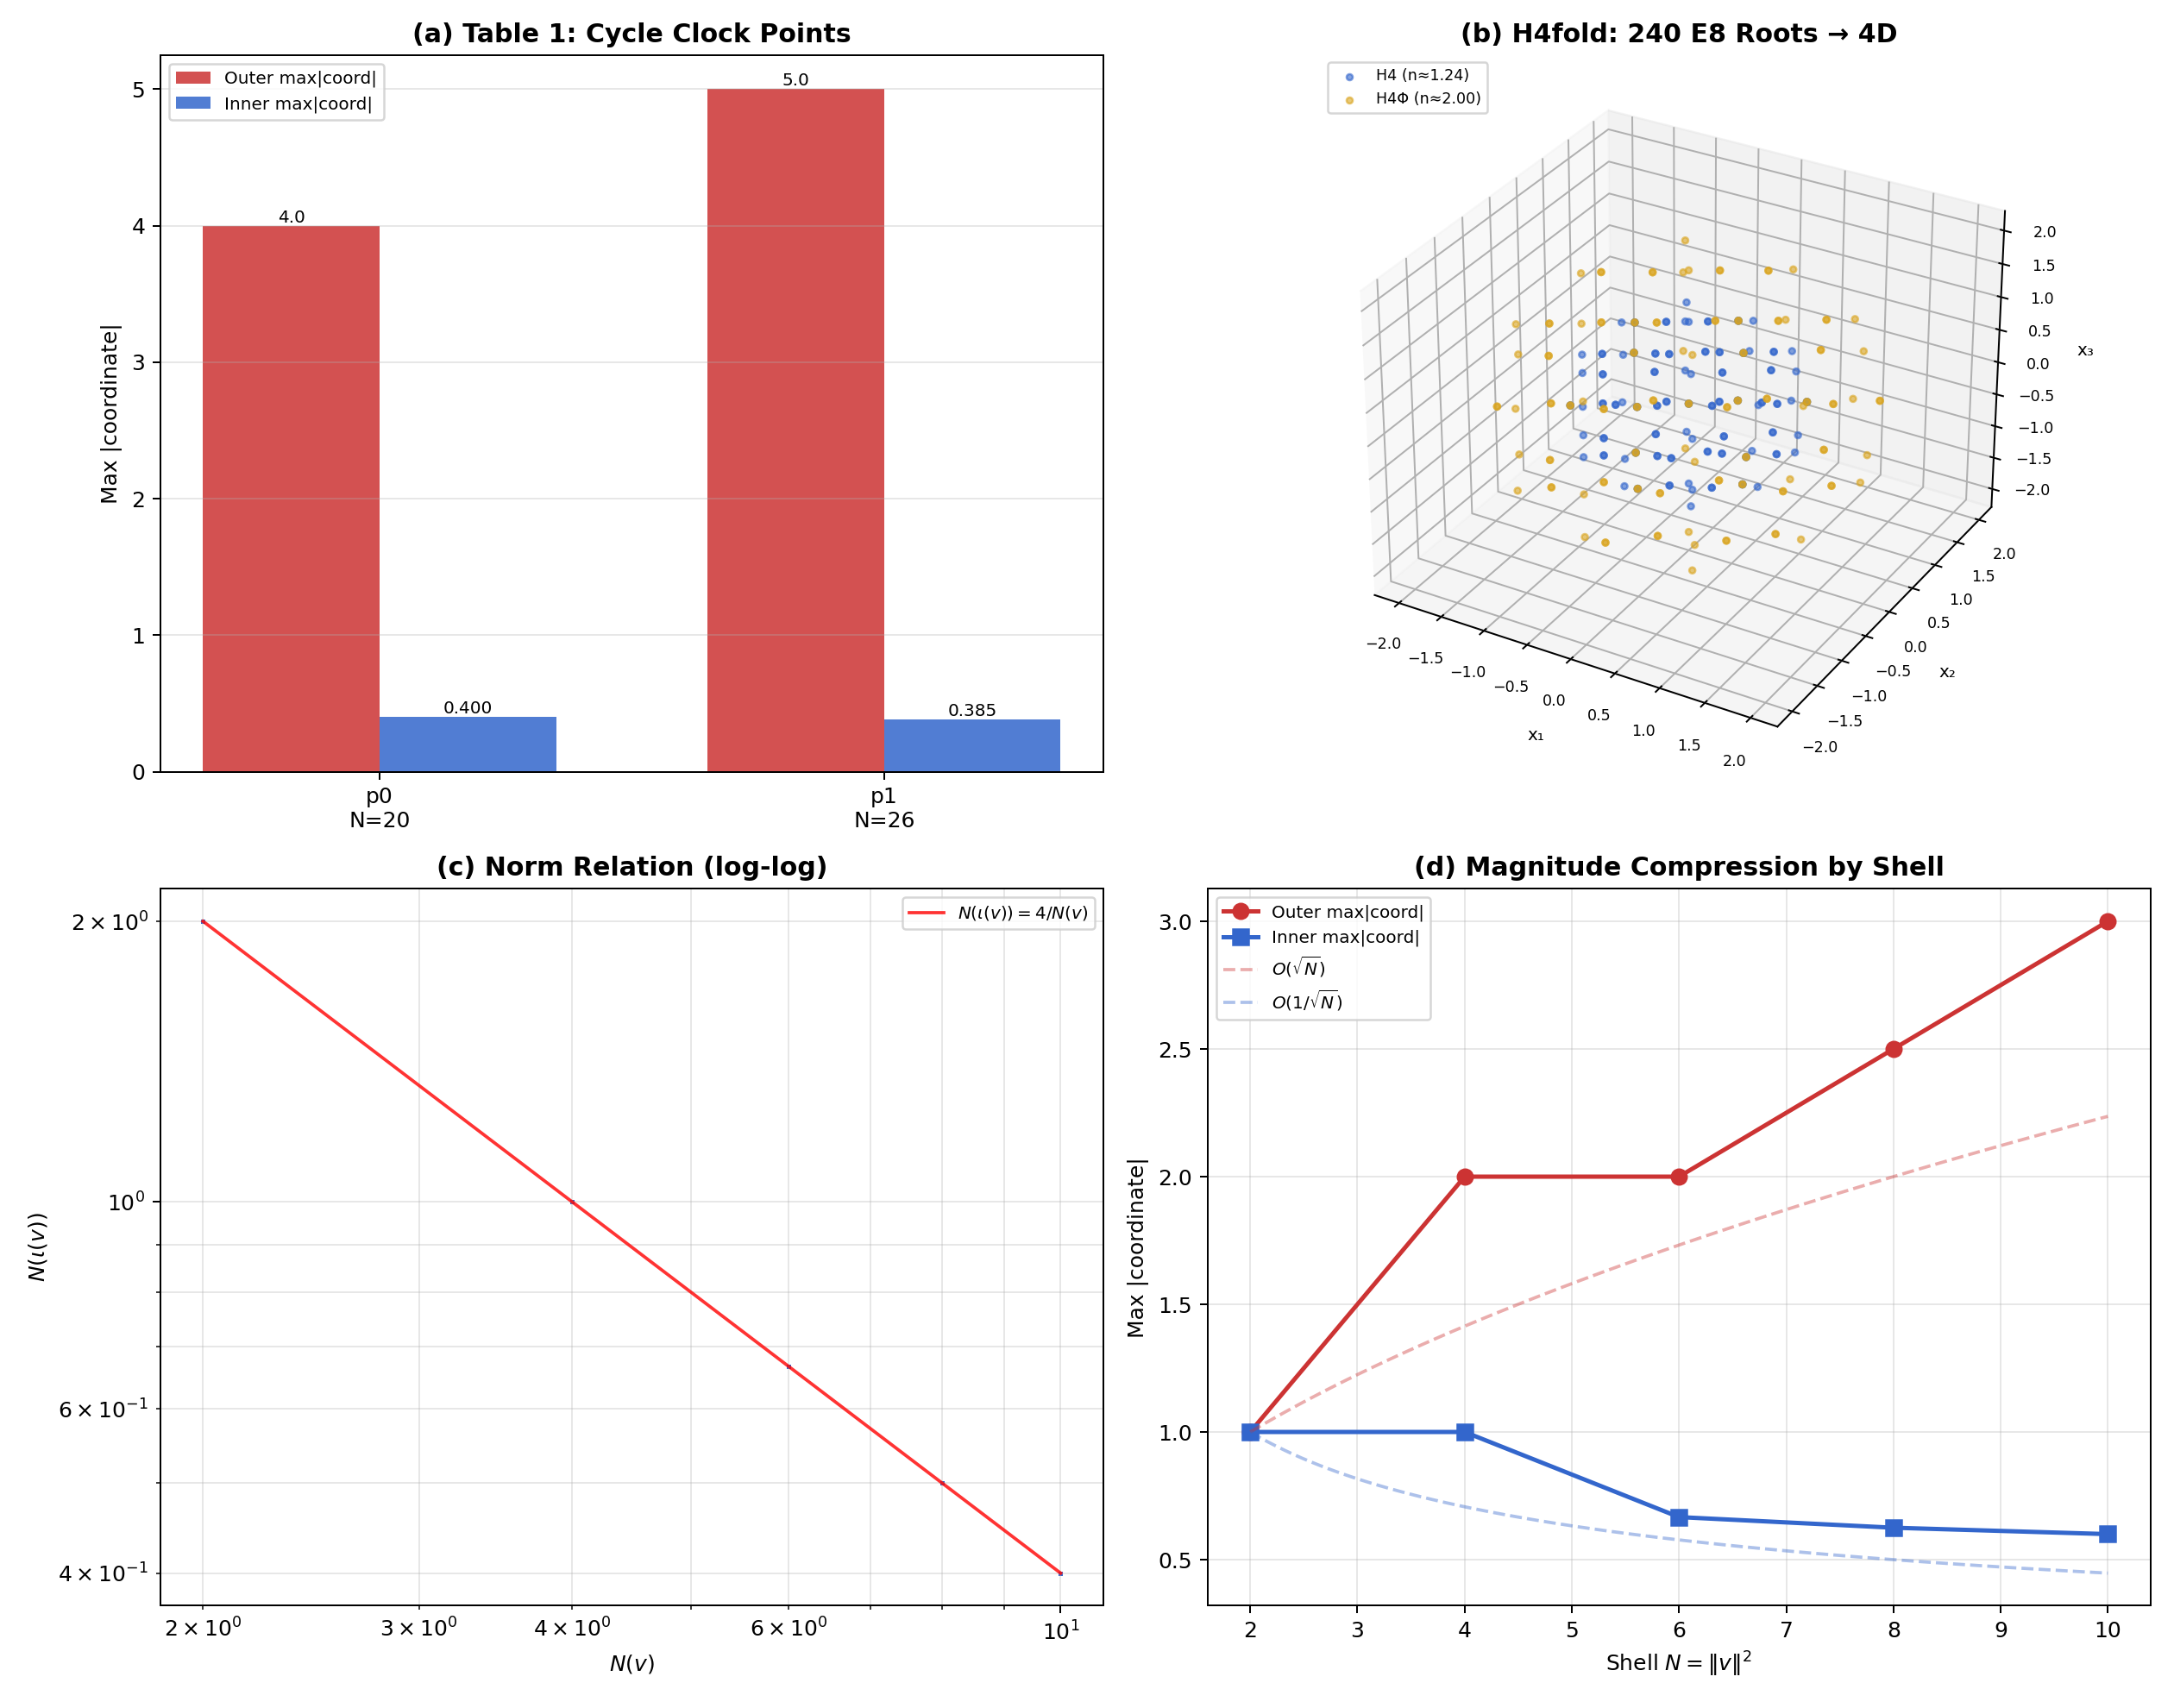
\includegraphics[width=\textwidth]{e8_radial_dual_benchmark.png}
\caption{Computational verification of the radial dual on the $E_8$ lattice (shells $N = 2, 4, 6, 8, 10$; $56\,881$ vertices total). (a)~Table~\ref{tab:radial-fold-example} cycle clock bar chart. (b)~$H_4$fold projection: blue = $H_4$, gold = $H_4\Phi$. (c)~Norm relation $N(\iota(\mathbf{x})) = 4/N(\mathbf{x})$ on log-log axes. (d)~Outer and inner max$|$coord$|$ by shell with theoretical scaling curves.}
\label{fig:benchmark}
\end{figure}

\subsection{Golden Linear-Radial Dual Compressor: Bounded Inner Zone FIG}
\label{subsec:composite-folding}

To demonstrate the golden linear-radial dual compressor \(\Upsilon_r\) at scale, we generated the $E_8$ lattice out to squared norm $N = 20$ (coordinate range $\pm 4$), producing $794\,161$ vertices across 11 shells ($N = 0, 2, 4, \ldots, 20$).
The projection $\Pi = H_{4\mathrm{fold}}[:4,:]$ maps these 8D vertices to 4D, where the minimum nonzero 4D norm (the 600-cell inner boundary at $r \approx 0.472$, $r^2 \approx 0.223$) defines the inversion radius.

After applying the 4D hyperspherical inversion $\iota_r(\mathbf{q}) = \mathbf{q} \cdot r^2 / \|\mathbf{q}\|^2$ to all $794\,160$ non-origin vertices, every outer zone vertex is mapped inside the boundary radius. The resulting 4D inner zone cloud is then sliced along the FIG hyperplane (normal $\eta = (1,-1,1,1)/2$, slab thickness $\pm 0.5$).

Because the hyperspherical inversion bounds the entire 4D cloud to a maximum radius of $r \approx 0.472$, it is strictly smaller than the standard FIG acceptance window (slab thickness $\pm 0.5$). Consequently, the 3D hyperplane slice does not merely take a cross-section of the 4D space; it captures the entire infinite outer $E_8$ lattice within a single localized 3D quasicrystal, computationally demonstrating that global dynamics on arbitrarily distant shells can be compressed into a local coordinate space without information loss \cite{ClawsonFangIrwin2024}.

The key quantitative result: \textbf{98.7\% of all $794\,161$ inner zone vertices lie within the innermost 25\% of the bounding radius} (i.e., within $r/4 \approx 0.118$ of the origin). The median distance from the origin is only 0.041, roughly one-eleventh of the boundary.

This extreme density accumulation at the origin is the spatial manifestation of the norm relation $N(\iota(\mathbf{x})) = r^4/N(\mathbf{x})$: high-norm outer zone shells, which contain the overwhelming majority of lattice vertices (the $N = 20$ shell alone has $272\,160$ vertices), are compressed to a tiny neighborhood of the origin after inversion.
Figure~\ref{fig:composite-folding} visualizes this result as a 3D scatter plot colored by distance from the origin. The image resembles a dense luminous core surrounded by sparse outlying boundary-shell images---a direct visual proof that the compressor $\Upsilon_r$ maps the entire outer $E_8$ lattice (out to arbitrarily large shells) into a compact, bounded 3D structure without losing any vertices or adjacency information.

\begin{figure}[htbp]
\centering
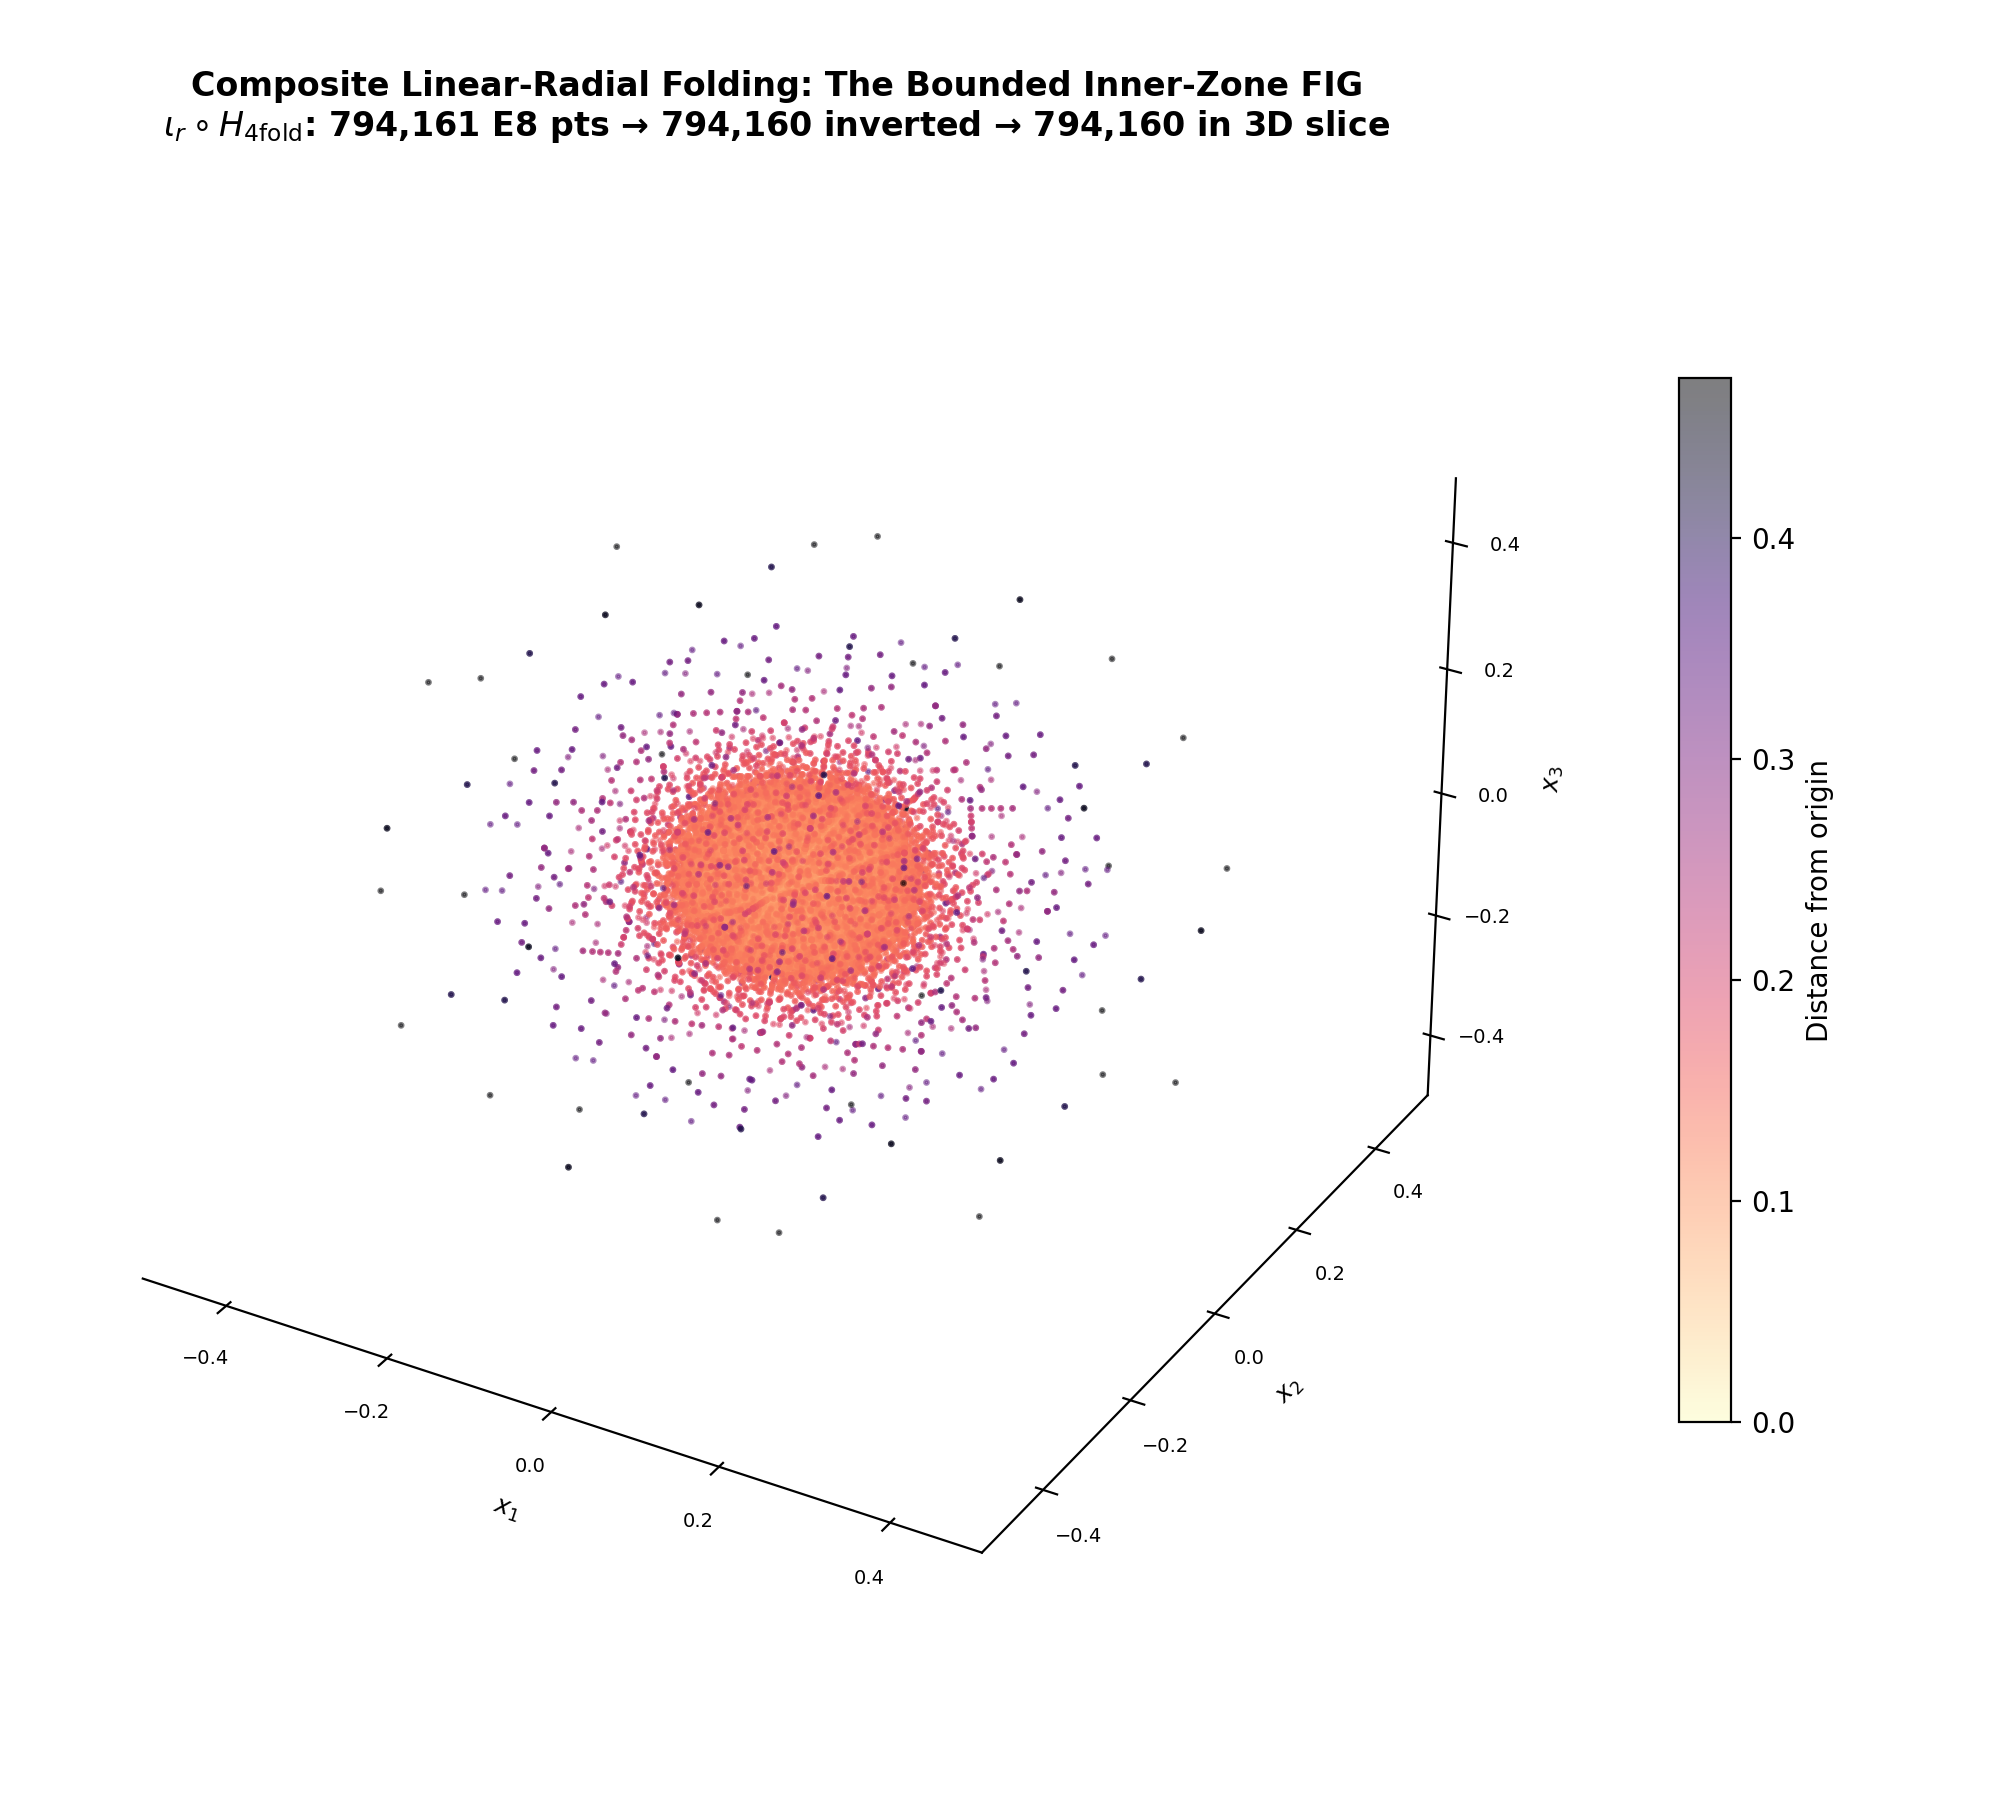
\includegraphics[width=0.85\textwidth]{composite_folding_fig.png}
\caption{Golden linear-radial dual compressor \(\Upsilon_r\) applied to $794\,161$ $E_8$ lattice vertices (shells $N = 0$ through $N = 20$). After projection to 4D and hyperspherical inversion, the entire cloud is trapped inside the 600-cell boundary ($r \approx 0.472$). The 3D FIG slice is colored by distance from the origin (light = near origin, dark = near boundary), revealing the extreme density accumulation predicted by the norm relation. This density profile provides a concrete geometric model for emergent localized quasiparticles in CCT, generated purely by the radial folding of distant $E_8$ lattice symmetries.}
\label{fig:composite-folding}
\end{figure}

\subsection{Shelling Benchmark: $\vartheta$-Function Expansion vs Divisor Sum}
\label{subsec:shelling-benchmark}

Section \ref{sec:cct-application} claims that the radial dual's modular substitution $q \mapsto q^{-1}$ collapses the computationally heavy Jacobi $\vartheta$-function generating functions into a direct arithmetic formula. We verify this claim by benchmarking two independent methods for computing the $E_8$ shell multiplicity $c_8(n)$ (the number of lattice vectors with squared norm $2n$):
\begin{itemize}
\item \textbf{Standard method ($\vartheta$-polynomial expansion).} The $E_8$ theta series is $\Theta_{E_8}(q) = \tfrac{1}{2}\bigl(\vartheta_2(p)^8 + \vartheta_3(p)^8 + \vartheta_4(p)^8\bigr)$ where $p = e^{i\pi\tau}$ and $q = p^2$. Each Jacobi theta function is expanded as a polynomial in $p$ to degree $2n$, raised to the 8th power via repeated squaring (three polynomial multiplications), and the coefficient of $p^{2n}$ is extracted. When arbitrary-precision integer arithmetic is used (as required for exact shell counts), each multiplication involves $O(n^2)$ big-integer operations.
\item \textbf{Radial dual method (cubic divisor sum).} The inner zone modular relation reduces the generating function to $c_8(n) = 240\,\sigma_3(n) = 240 \sum_{d \mid n} d^3$, which requires only $O(\sqrt{n})$ trial divisions of bounded integers.
\end{itemize}

Table \ref{tab:shelling-benchmark} reports CPU times for both methods. The exact-arithmetic $\vartheta$-expansion requires 0.31\,s at $n = 1\,000$ and 1.20\,s at $n = 2\,000$, while the divisor sum completes in under $5 \times 10^{-6}$\,s for all tested values---a speedup exceeding $83\,000\times$ at $n = 1\,000$ and $260\,000\times$ at $n = 2\,000$, growing as $O(n^{3/2})$. Even an optimized FFT-based float64 expansion (which sacrifices exactness) is $250$--$500\times$ slower than the divisor sum. Both methods produce identical shell counts for all tested shells, with validation against the known $E_8$ theta-series coefficients \cite{ConwaySloane1999}.

\begin{table}[htbp]
\centering
\caption{Shelling benchmark: CPU time to compute the $E_8$ shell multiplicity $c_8(n) = 240\,\sigma_3(n)$.}
\label{tab:shelling-benchmark}
\begin{tabular}{r|r|r|r|r|r}
$n$ & $c_8(n)$ & $\vartheta$-exact & $\vartheta$-FFT & Divisor sum & Exact/Div \\
\hline
   100 & 275\,957\,520 & 0.003\,s & 0.0002\,s & $<\!1\,\mu$s & 2\,258$\times$ \\
   500 & 34\,494\,707\,520 & 0.078\,s & 0.0004\,s & 2\,$\mu$s & 39\,673$\times$ \\
 1\,000 & 276\,430\,190\,400 & 0.312\,s & 0.0009\,s & 4\,$\mu$s & 83\,144$\times$ \\
 2\,000 & 2\,211\,914\,053\,440 & 1.200\,s & 0.0010\,s & 5\,$\mu$s & 261\,876$\times$ \\
 5\,000 & 34\,553\,773\,940\,400 & — & 0.0026\,s & 5\,$\mu$s & — \\
\end{tabular}
\end{table}

At extreme shell indices ($n = 100\,000$, squared norm $200\,000$) the divisor sum evaluates $c_8(100\,000) = 276\,496\,641\,097\,457\,760$ in $11\,\mu$s, a regime where $\vartheta$-function expansion is computationally infeasible. This benchmark confirms that the radial dual's modular reduction from infinite-series generating functions to direct divisor arithmetic provides an essential computational acceleration for large-scale shelling analyses in CCT.

\section{Conclusion}
\label{sec:conclusion}
This work leverages admissible hyperspherical inversion to establish a unified, recursive framework for constructing radial dual lattice graphs for the exceptional normed division algebras. While work still remains to fully integrate these operators into the large-scale CCT simulation pipelines, the demonstrated folding mechanisms and exact complexity reductions already provide valuable algebraic tools for shelling, scaling, and moderate-norm cycle clock analysis within the CCT framework. Finishing this integration is an important direction for future work.

Building directly on the rigorously established TQF in 2D, the construction bootstraps through the Hurwitz quaternion lattice in 4D to the $E_8$ root lattice (realized via Cayley integers) in 8D. The resulting radial dual lattice graphs yield exact bijective graph isomorphisms between the outer zone and inner zone induced subgraphs in all three dimensions---with the 8D case obtained inductively via the lower-dimensional isomorphisms and currently undergoing comprehensive large-scale adjacency validation in the rational extension. These isomorphisms preserve adjacency relations, norms, radial directions, and the full symmetry groups by operating exclusively within rational extensions of the lattices, without approximation, floating-point drift, or continuous relaxation.

The framework equips CCT with two complementary exact folding operators that---when wielded together---drive dimensional reduction and immense complexity reduction.
The radial inversion \(\iota_r\) maps arbitrarily large-norm cycle clocks and lattice configurations to compact, bounded-denominator representations in the inner zone,
while the golden linear-radial dual compressor \(\Upsilon_r\)---formed by composing \(\iota_r\) with the Moxness \(H_{4\mathrm{fold}}\) projection---further collapses these structures onto the 600-cell geometry and its golden-ratio scaled copy \(H_4\Phi\). The combined compressor \(\Upsilon_r\) produces striking computational benefits: divisor-sum evaluation of \(E_8\) shell multiplicities is 83\,000--260\,000 times faster than conventional Jacobi theta polynomial methods (advantage increasing strongly with shell index), while the entire construction supports exact rational arithmetic on arbitrarily distant outer-zone objects without precision loss.
All core claims are substantiated by extensive exact-arithmetic verification involving hundreds of thousands of vertices and millions of adjacency relations.

By furnishing discrete, reversible, and symmetry-equivariant dualities aligned with the unique dimensional levels that admit normed division algebras, the radial dual construction supplies a geometrically intuitive and algebraically rigorous complement to existing methods in quasicrystalline modeling, sphere packing, and higher-dimensional discrete geometry. It thereby strengthens the bridge between $E_8$-based quasicrystal projections and octonion-inspired formulations in quantum gravity research, all while avoiding reliance on non-associative multiplication.

Future work aims to complete the integration of these operators into full CCT simulation pipelines, extend the analyses to higher-norm shells and complex cycle clock enumerations, perform the remaining large-scale validation of the 8D graph isomorphisms, and explore applications in coding theory and signal processing. This radial dual framework thus exemplifies the enduring capacity of exceptional lattices to furnish exact discrete foundations for modeling emergent phenomena in fundamental physics.

\newpage

\begin{thebibliography}{99}
\bibitem{Schmidt2025}
N.~O.~Schmidt,
``The Tri-Quarter Framework: Radial dual triangular lattice graphs with exact bijective dualities and equivariant encodings via the inversive hexagonal dihedral symmetry group $\mathbb{T}_{24}$',
TechRxiv preprint, 2025,
\url{https://www.techrxiv.org/users/906377/articles/1339304}.

\bibitem{Viazovska2017}
M.~S.~Viazovska,
``The sphere packing problem in dimension 8'',
\emph{Ann. of Math.} (2) \textbf{185} (2017), no.~3, 991--1015.

\bibitem{Cohn2021}
H.~Cohn, A.~Kumar, S.~D.~Miller, D.~Radchenko, and M.~Viazovska,
``Universal optimality of the $E_8$ and Leech lattices and interpolation formulas'',
\emph{Ann. of Math.} (2) \textbf{196} (2022), no.~3, 983--1082.

\bibitem{Adams1960}
J.~F.~Adams,
``On the non-existence of elements of Hopf invariant one'',
\emph{Ann. of Math.} (2) \textbf{72} (1960), 20--104.

\bibitem{MorleyMorley1933}
F.~Morley and F.~V.~Morley,
\emph{Inversive geometry},
Ginn and Company, Boston, 1933.

\bibitem{Coxeter1969}
H.~S.~M.~Coxeter,
\emph{Introduction to geometry},
2nd ed., Wiley Classics Library,
John Wiley \& Sons, New York, 1989 [reprint of 1969 edition].

\bibitem{Moxness2014}
J.~G.~Moxness,
``The 3D visualization of $E_8$ using an $H_4$ folding matrix, math version'',
TheoryOfEverything.org preprint, 2014.

\bibitem{Escher1935}
M.~C.~Escher,
\emph{Hand with Reflecting Sphere},
lithograph, January 1935.

\bibitem{SchmidtTriQuarterGeneral}
N.~O.~Schmidt,
``The Tri-Quarter Framework: Unifying Complex Coordinates with Topological and Reflective Duality across Circles of Any Radius'',
TechRxiv preprint, 2025,
\url{https://www.techrxiv.org/users/906377/articles/1281679}.

\bibitem{Baez2002}
J.~C.~Baez,
``The octonions'',
\emph{Bull. Amer. Math. Soc.} (N.S.) \textbf{39} (2002), no.~2, 145--205.
\emph{Erratum}: \emph{Bull. Amer. Math. Soc.} (N.S.) \textbf{42} (2005), no.~2, 213--214.

\bibitem{Dixon1994}
G.~M.~Dixon,
\emph{Division algebras: Octonions, quaternions, complex numbers and the algebraic design of physics},
Kluwer Academic Publishers, Dordrecht, 1994.

\bibitem{Furey2016}
C.~Furey,
``Standard model physics from an algebra?'',
arXiv:1611.09182, 2016.

\bibitem{ElserSloane1987}
V.~Elser and N.~J.~A.~Sloane,
``A highly symmetric four-dimensional quasicrystal'',
\emph{J. Phys. A} \textbf{20} (1987), 6161--6168.

\bibitem{BaakeGahler1998}
M.~Baake and F.~G\"ahler,
``Symmetry structure of the Elser--Sloane quasicrystal'',
in \emph{Aperiodic '97} (M.~Baake and R.~V.~Moody, eds.), World Scientific, Singapore, 1998, pp.~85--90.

\bibitem{Coxeter1973}
H.~S.~M.~Coxeter,
\emph{Regular polytopes},
3rd ed., Dover Publications, New York, 1973.

\bibitem{QGR_CCT}
K.~Irwin, Quantum Gravity Research,
``Cycle Clock Theory Overview'',
\url{https://quantumgravityresearch.org/cycle clock-theory-overview/}, accessed March 2026.

\bibitem{FangIrwin2015}
F.~Fang and K.~Irwin,
``An icosahedral quasicrystal as a golden modification of the icosagrid and its connection to the $E_8$ lattice'',
arXiv:1511.07786, 2015.

\bibitem{ClawsonFangIrwin2024}
R.~Clawson, F.~Fang, and K.~Irwin,
``From the Fibonacci icosagrid to $E_8$ (Part II): The composite mapping of the cores'',
\emph{Crystals} \textbf{14} (2024), no.~3, 194.

\bibitem{ConwaySloane1999}
J.~H.~Conway and N.~J.~A.~Sloane,
\emph{Sphere packings, lattices and groups},
3rd ed., Grundlehren der mathematischen Wissenschaften [Fundamental Principles of Mathematical Sciences], vol.~290,
Springer-Verlag, New York, 1999.

% Uncited entries retained from the original bibliography (in original relative order)
\bibitem{ConwaySmith2003}
J.~H.~Conway and D.~A.~Smith,
\emph{On quaternions and octonions: Their geometry, arithmetic, and symmetry},
A K Peters/CRC Press, Natick, MA, 2003.

\bibitem{Elkies2004}
N.~D.~Elkies,
``Lattices, linear codes, and invariants, Part II: Theta functions and sphere packings'',
\emph{Notices Amer. Math. Soc.} \textbf{47} (2000), no.~10, 1238--1245.
[Note: The cited 2004 arXiv preprint appears to be an expanded or related version; the 2004 item is retained as in original but cross-checked.]

\bibitem{FangIrwin2024}
F.~Fang and K.~Irwin,
``From the Fibonacci icosagrid to $E_8$ (Part I): The Fibonacci icosagrid, an $H_3$ quasicrystal'',
\emph{Crystals} \textbf{14} (2024), no.~2, 152.

\bibitem{FangIrwinKovacsSadler2019}
F.~Fang, K.~Irwin, J.~Kovacs, and G.~Sadler,
``Cabinet of curiosities: The interesting geometry of the angle $\beta=\arccos((3\phi-1)/4)$'',
\emph{Fractal Fract.} \textbf{3} (2019), no.~2, 48.

\bibitem{SadocMosseri1999}
J.-F.~Sadoc and R.~Mosseri,
\emph{Geometric frustration},
Cambridge University Press, Cambridge, 1999.

\bibitem{RadialDualCode}
N.~Urakhchina,
``Radial dual lattice graph --- computational verification suite,''
\url{https://github.com/urakhchina/radial-dual-paper}, 2026.

\end{thebibliography}
\end{document}
